\newif\iffunny
\funnyfalse

\documentclass[xcolor={dvipsnames}]{beamer}
\usepackage{color, colortbl}
\usepackage[ngerman,english]{babel}
\usepackage[T1]{fontenc}
\usepackage{CJKutf8} %japanese
\usepackage{lmodern}
%\usepackage{subfigure}
\usepackage[compatibility=false]{caption}
\usepackage{subcaption}
\usepackage{tikz}
\usepackage{textgreek}
\usepackage{tabularx}
\usepackage{booktabs}
\usepackage{siunitx}
\usepackage{appendixnumberbeamer}
\usepackage[absolute,overlay]{textpos} %for positioning the logos where I want

\usepackage{animate}
\usepackage{multimedia}

\mode<presentation>
{
  \usetheme{CambridgeUS}     
  \usecolortheme{lily} 
  \definecolor{beamer@violet}{rgb}{0.5,0.3,0.5} % changed this
  \setbeamercolor{structure}{fg=beamer@violet!70!cyan}
  \setbeamercolor{palette primary}{fg=black, bg=gray!30!white!50!cyan!20!}
  \setbeamercolor{palette secondary}{fg=black, bg=gray!30!white!30!cyan!40!}
  \setbeamercolor*{palette tertiary}{bg=gray!20!white!20!cyan!60!}
  
  \setbeamercolor{frametitle}{fg=cyan!60!white!40!,bg=cyan!80!black}
  \setbeamercolor{title}{fg=cyan!80!black}
  \setbeamercolor{normal text}{fg=black,bg=white}
  \setbeamercolor{alerted text}{fg=beamer@violet}
  \setbeamercolor{example text}{fg=beamer@violet!70!cyan}
  
  \usefonttheme{structureitalicserif} 
  \setbeamertemplate{navigation symbols}{}
  \setbeamertemplate{caption}[numbered]
}
\newcommand{\sidlogo}{
  \setlength{\TPHorizModule}{1pt}
  \setlength{\TPVertModule}{1pt}
   % textblock{}{x,y}: pos(x) = rightUpperCorner + (x * \TPHorizModule), pos(y) = leftUpperCorner - (y * \TPVertModule)
  \begin{textblock}{1}(323,12)
   
\includegraphics[width=40pt,height=26pt]{figures/SiD.jpeg}
  \end{textblock}
  } 
\newcommand{\ilclogo}{
  \setlength{\TPHorizModule}{1pt}
  \setlength{\TPVertModule}{1pt}
   % textblock{}{x,y}: pos(x) = rightUpperCorner + (x * \TPHorizModule), pos(y) = leftUpperCorner - (y * \TPVertModule)
  \begin{textblock}{1}(323,12)
   
\includegraphics[width=40pt,height=26pt]{figures/ILC.jpeg}
  \end{textblock}
} 
\newcommand{\ejadelogo}{
  \setlength{\TPHorizModule}{1pt}
  \setlength{\TPVertModule}{1pt}
   % textblock{}{x,y}: pos(x) = rightUpperCorner + (x * \TPHorizModule), pos(y) = leftUpperCorner - (y * \TPVertModule)
  \begin{textblock}{1}(323,12)
   
\includegraphics[width=40pt,height=26pt]{figures/EJADE.jpeg}
  \end{textblock}
} 


\title[ILC \& Background Simulations]{\textbf{\LARGE The International Linear Collider \\ \normalsize- \\ \small Background Simulations \& Optimizing the Final Focus Region}}
\author{\textbf{Anne Sch\"utz}}
\institute{\textbf{KIT, DESY}}
\date{\textbf{18. February 2016}}

\titlegraphic{
\includegraphics[height=1.0cm]{figures/KIT.png}\hspace*{6cm}~%
   
\includegraphics[height=1.2cm]{figures/DESY_Logo.png}
}

\begin{document}

{
\usebackgroundtemplate{
 \tikz\node[opacity=0.1]{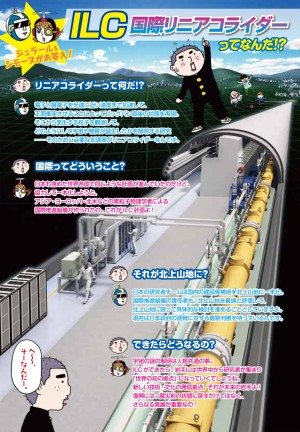
\includegraphics[width=\paperwidth]{figures/Iwatecomics.jpg}};
 % \tikz\node[opacity=0.2]{\centering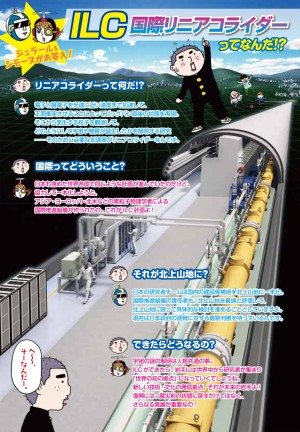
\includegraphics[height=\paperheight]{figures/Iwatecomics.jpg}};
 }
\begin{frame}
  \titlepage
\end{frame}
}

\begin{frame}{Table of contents}
  \tableofcontents
\end{frame}

\section{My Ph.D topic and myself}
\subsection{About me}

\begin{frame}{About me}
\begin{columns}
\begin{column}[T]{0.6\textwidth}
Anne Sch\"utz\\
\begin{itemize}
\item Studied Physics at KIT
\item Master's Thesis at DESY: \\ \textit{Simulating the Particles Fluxes at the DESY-II Test Beam Facility}
\item Since April 2015: Ph.D Thesis at DESY
\end{itemize}
\vspace*{0.7cm}
My supervisors\\
\begin{itemize}
\item Prof. Dr. G\"unter Quast (KIT)
\item Prof. Dr. Eckhard Elsen (CERN)
\item Dr. Marcel Stanitzki (DESY)
\end{itemize}
\end{column}

\begin{column}[T]{0.35\textwidth}
\vspace{0pt}%
\centering
	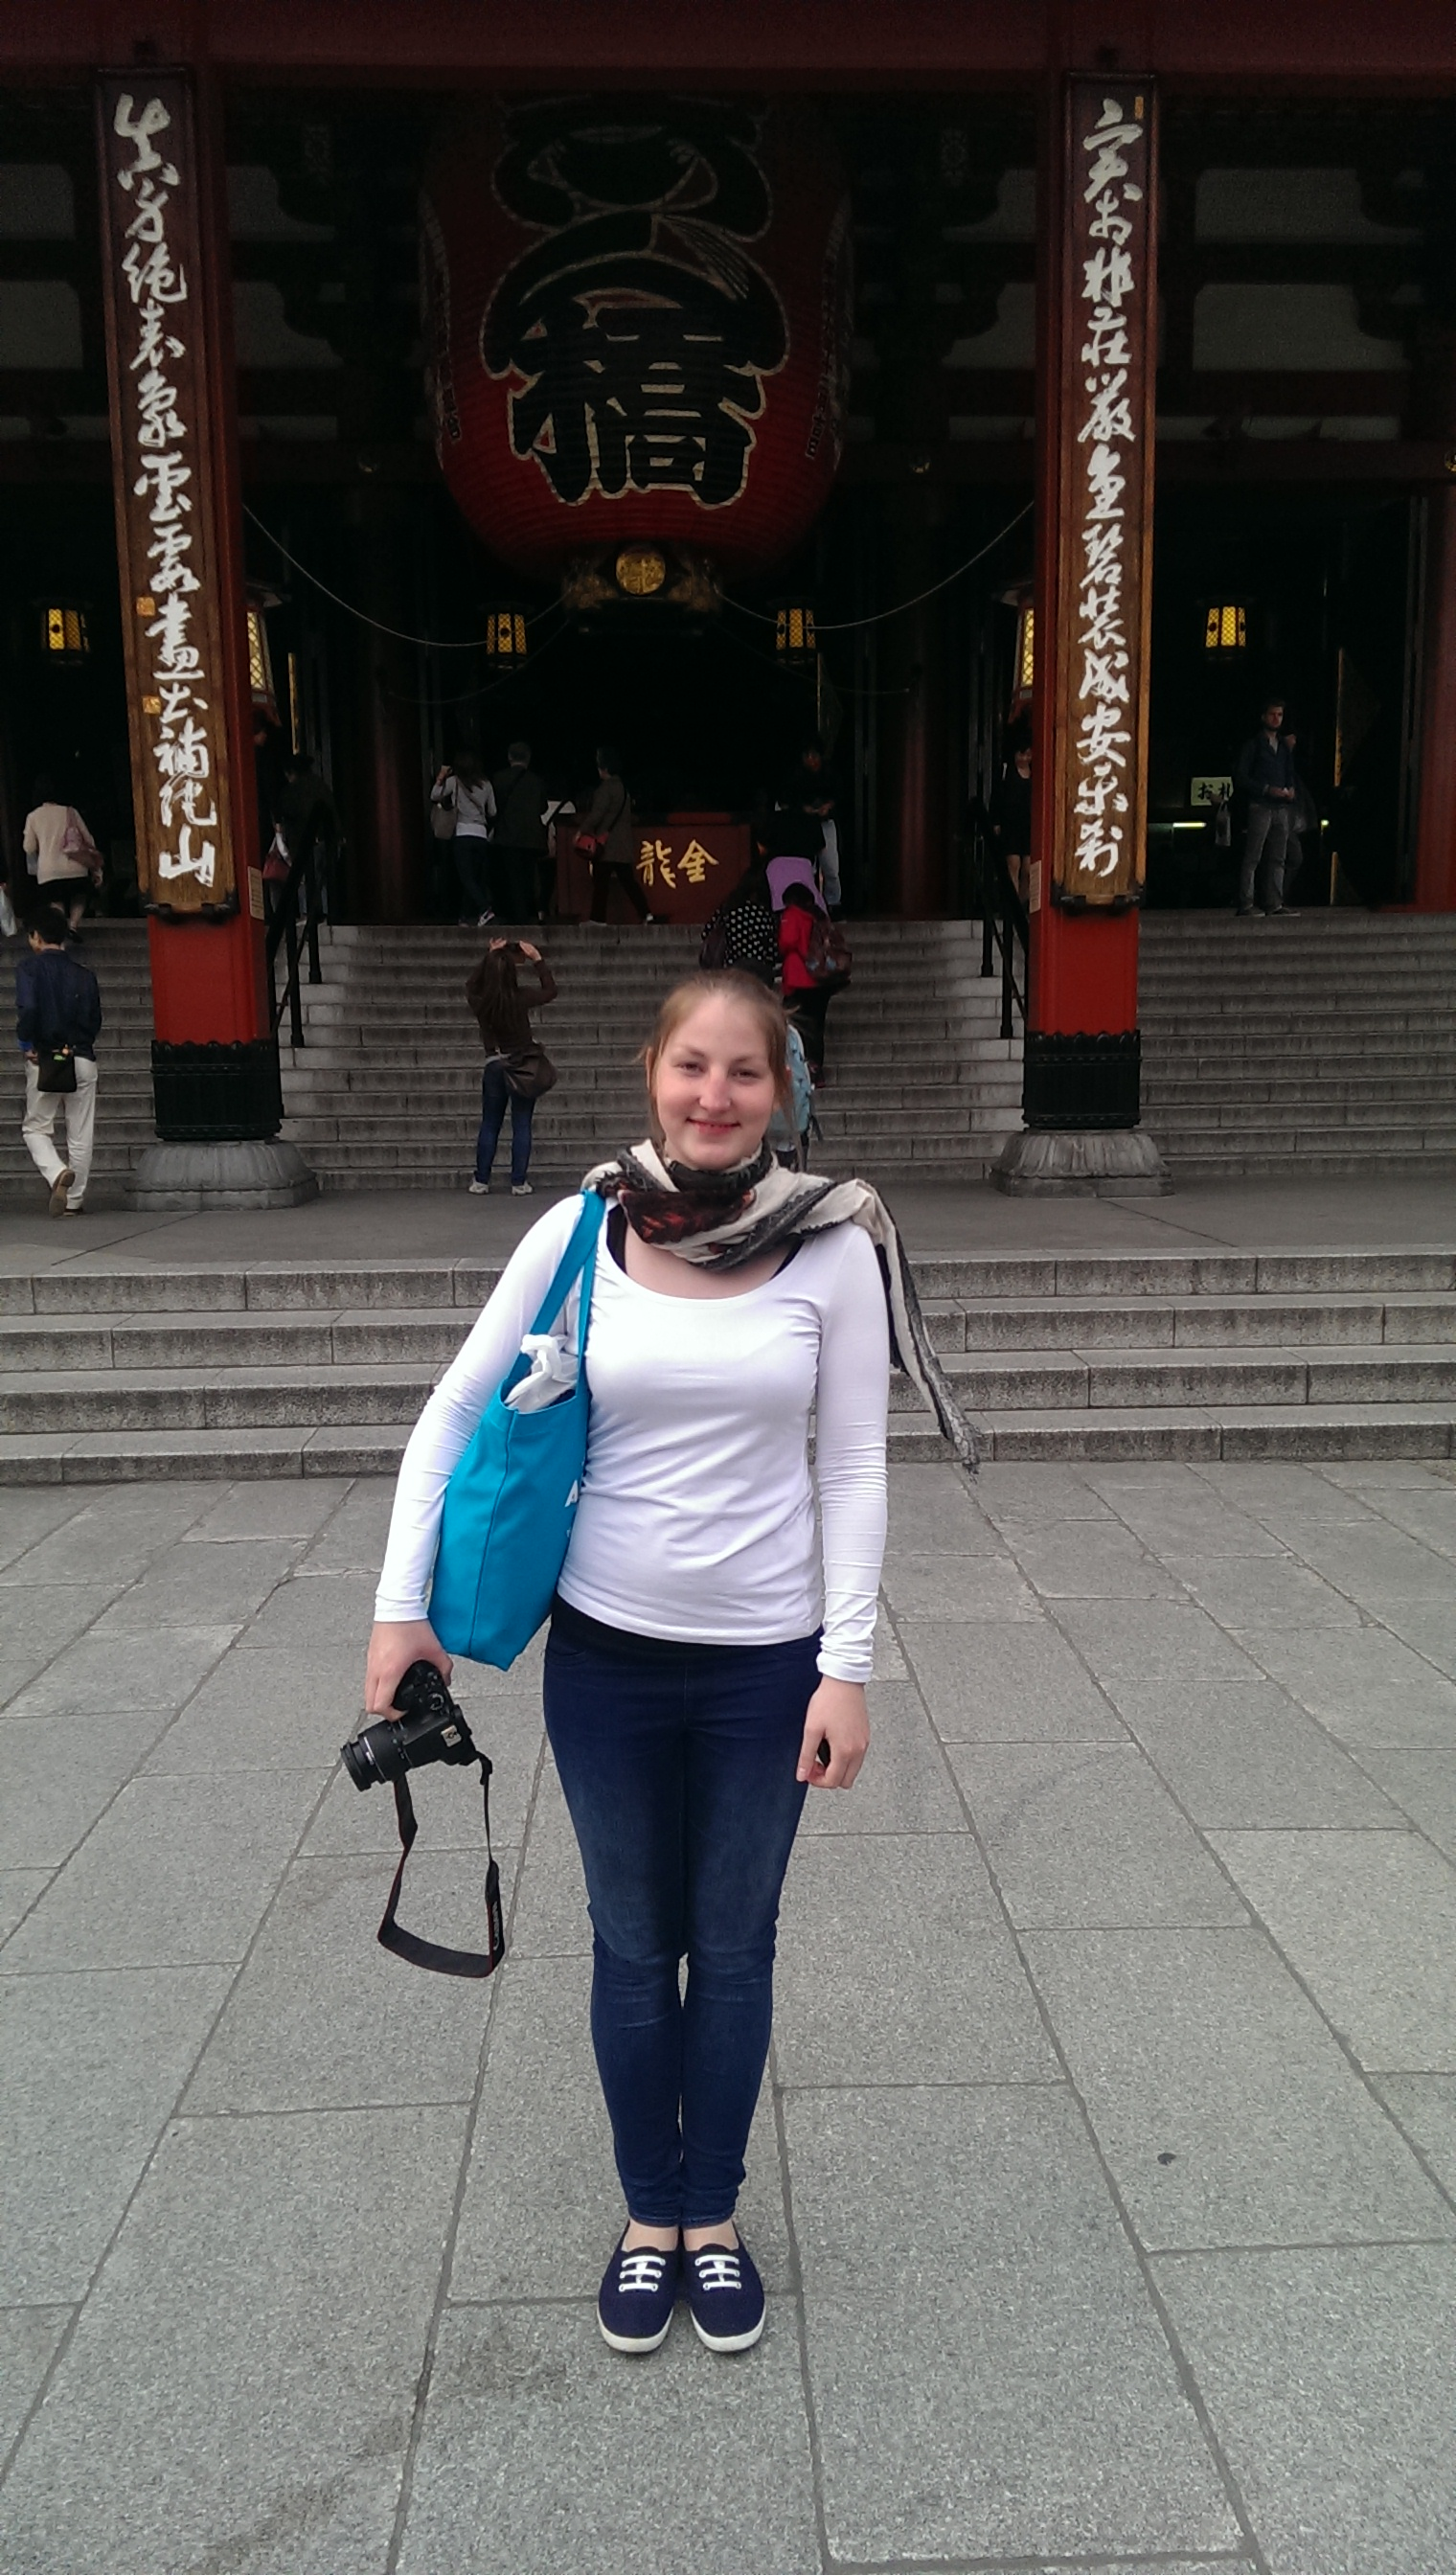
\includegraphics[width=0.7\textwidth]{figures/Myself_inJapan.jpg}
\end{column}
\end{columns}

\end{frame}

\subsection{My Ph.D topic}
\begin{frame}{My Ph.D topic}
\ilclogo
\begin{center}
\visible<3->{
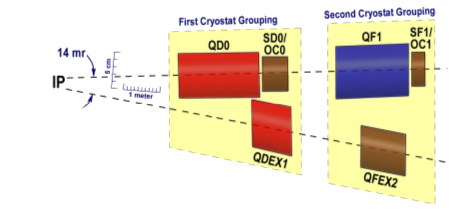
\includegraphics[width=0.4\textwidth]{figures/ILCTDR-VOLUME_3-PART_II_FFRegion.png}
}
\begin{block}{}
\centering
\textit{Optimizing the design of the Final-Focus Region\\for the International Linear Collider}
\end{block}
\visible<2->{
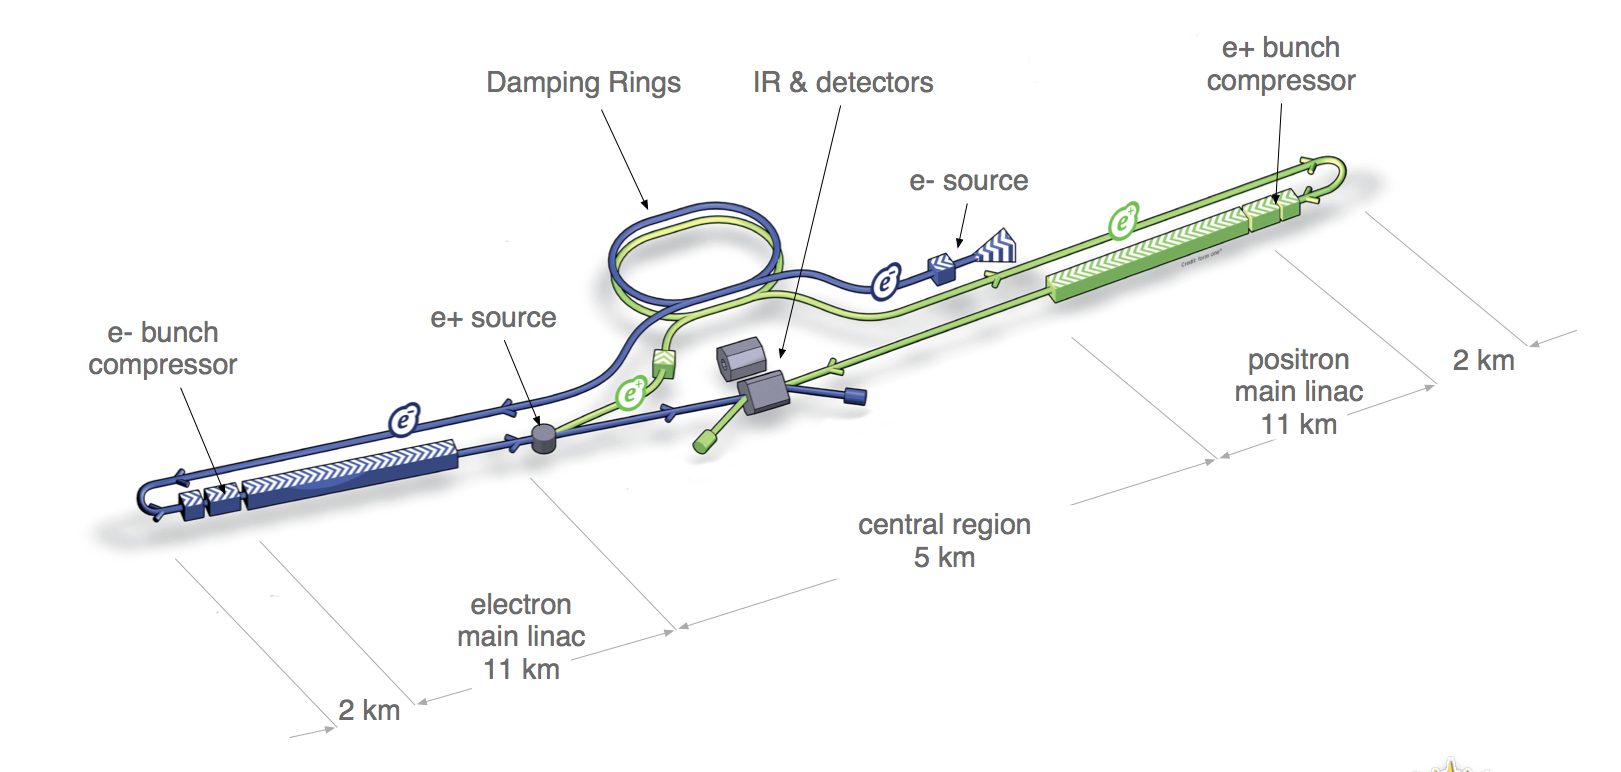
\includegraphics[width=0.7\textwidth]{figures/ILC_schematic_layout.png}
}
\end{center}
\end{frame}

\section{The International Linear Collider}
\subsection{Site}

\begin{frame}{The site of the ILC - The Kitakami mountains}
\ilclogo
\begin{center}
\only<1>{
\begin{tikzpicture}[every node/.style={anchor=center}]
 \node(b) at (16,8){
\begin{minipage}[t]{0.49\textwidth}
\centering
 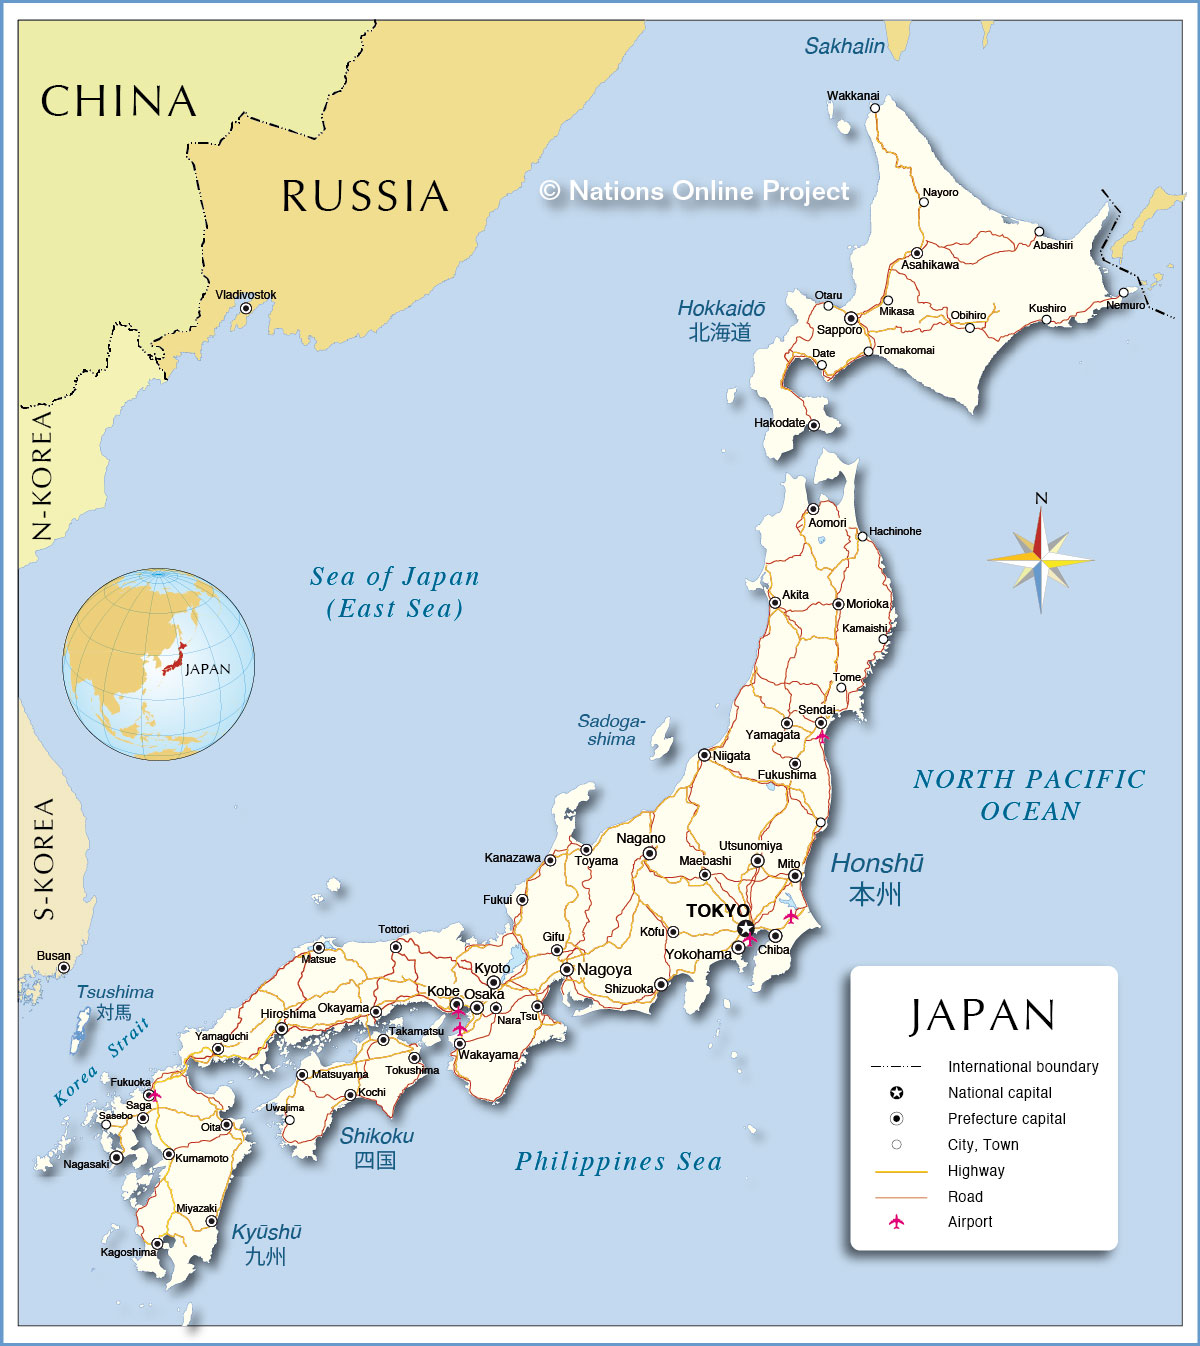
\includegraphics[width=\textwidth]{figures/japan-map.jpg}
\end{minipage}
\begin{minipage}[t]{0.48\textwidth}
\centering
   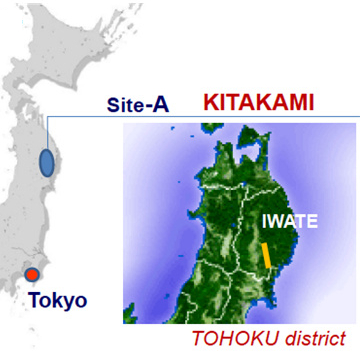
\includegraphics[width=\textwidth]{figures/Kitakami_site.jpg}
\end{minipage}
};
\end{tikzpicture}
}
	\iffunny 
\only<2>{
 \begin{tikzpicture}[every node/.style={anchor=center}]
  \node(b) at (16,8){
\begin{minipage}[t]{0.49\textwidth}
\centering
 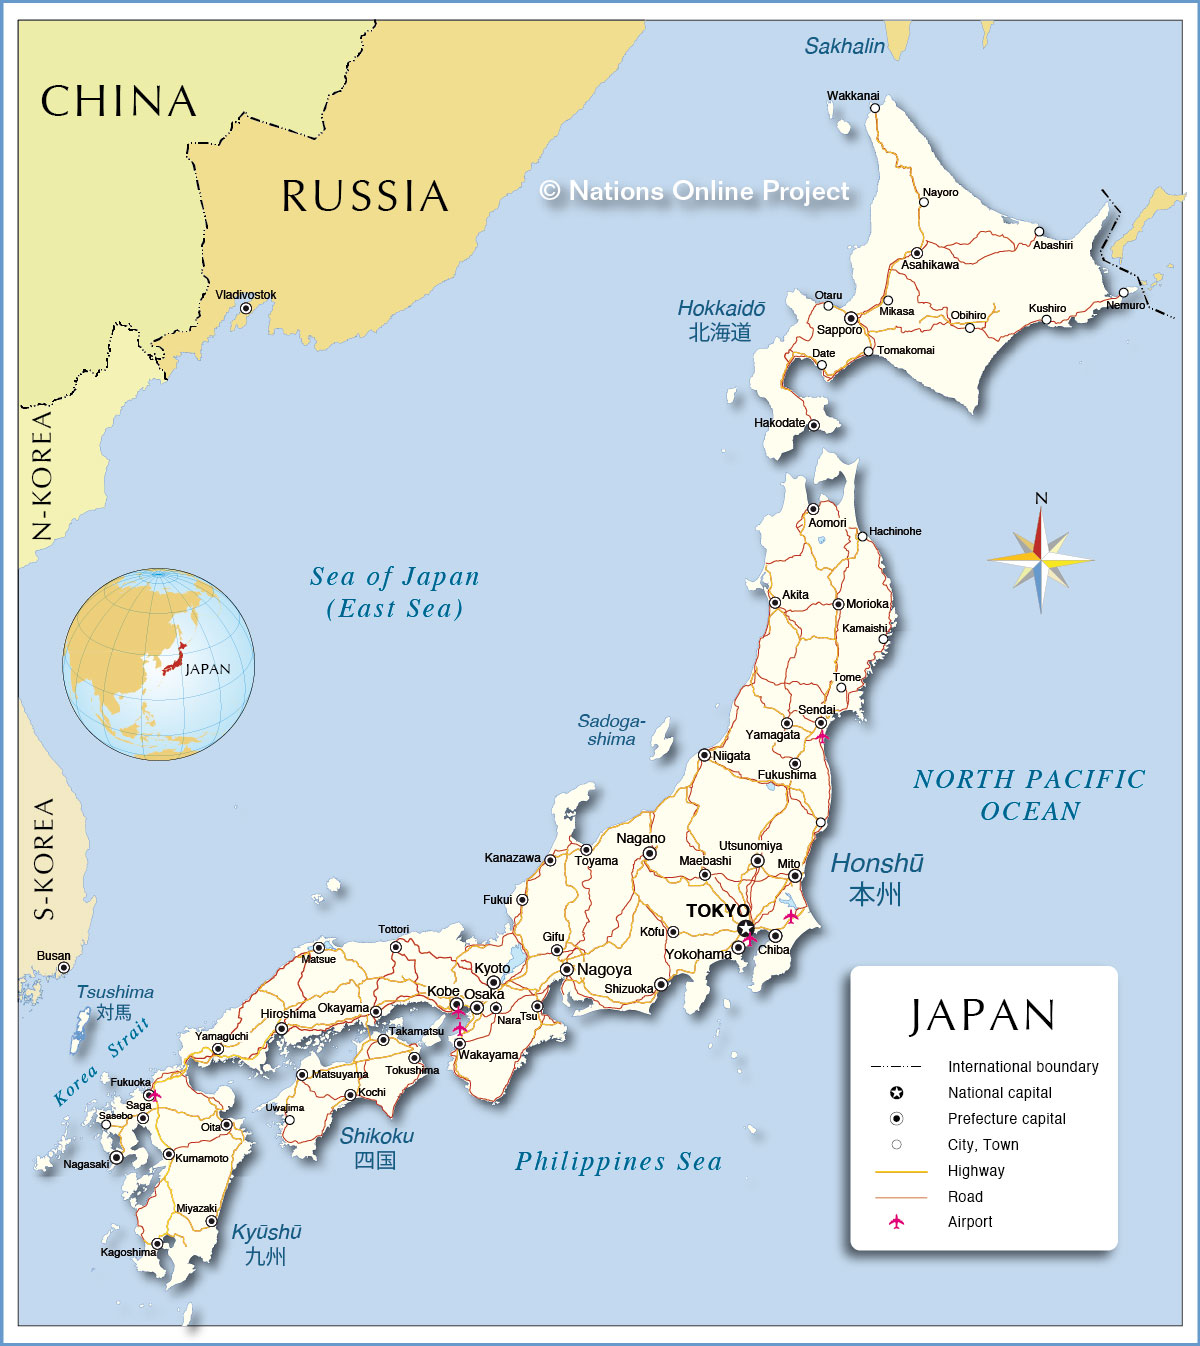
\includegraphics[width=\textwidth]{figures/japan-map.jpg}
\end{minipage}
\begin{minipage}[t]{0.48\textwidth}
\centering
   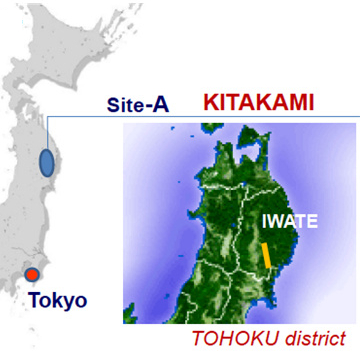
\includegraphics[width=\textwidth]{figures/Kitakami_site.jpg}
\end{minipage}
};
    \pause
   		\node(b) at (16,8){\includegraphics[width=0.3\textwidth]{figures/japaneseMyself.png}};
  \end{tikzpicture}
}
	\fi
\end{center}
\end{frame}

\subsection{The layout}
\begin{frame}{The layout of the ILC}
\ilclogo

e$^+$e$^-$ linear collider with adjustable center-of-mass energy, and polarized beams\\
\begin{center}
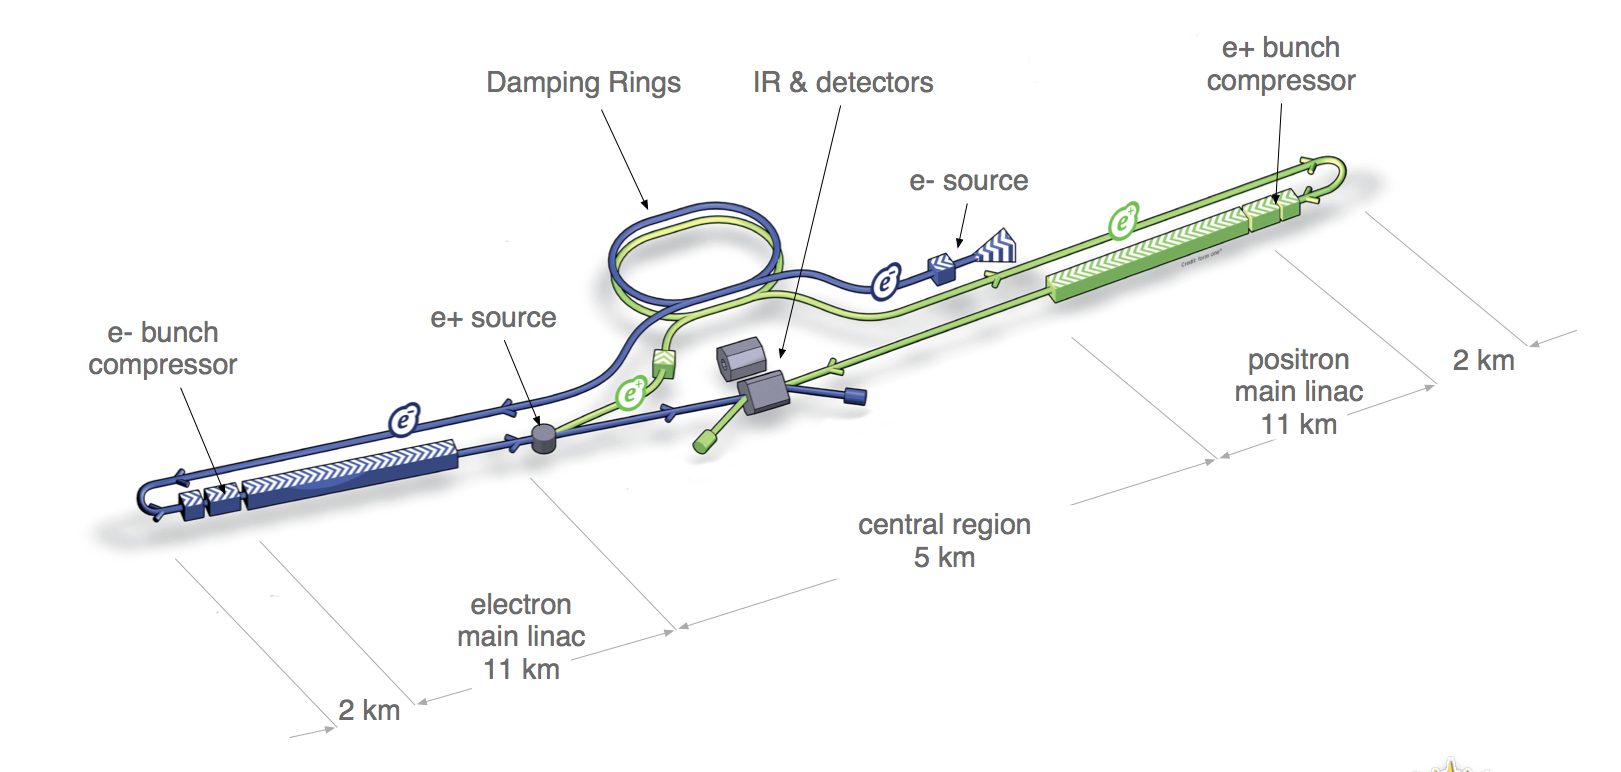
\includegraphics[width=\textwidth]{figures/ILC_schematic_layout.png}
\end{center}
\begin{flushright}
 \href{https://www.youtube.com/watch?v=ep5496vdEFI}{\beamergotobutton{\begin{CJK}{UTF8}{min}国際リニアコライダー\end{CJK}}}
\end{flushright}

\end{frame}

\begin{frame}{Why linear?}
\begin{columns}
 \begin{column}{0.6\textwidth}
  Basic limitations of lepton synchrotons:
\begin{itemize}
 \item \textcolor{Red}{Energy loss due to synchrotron radiation: $\sim$ E$^4$/R}
 \item \textcolor{Red}{Cost $\sim$ quadratically with energy}\\ \tiny{(B. Richter 
1980)}
\end{itemize}
\vspace*{1cm}
Therefore a linear collider:
\begin{itemize}
 \item \textcolor{ForestGreen}{Not limited by synchrotron radiation}
 \item \textcolor{ForestGreen}{Cost $\sim$ linear with energy}
\end{itemize}
 \end{column}
 \begin{column}{0.4\textwidth}
 \begin{block}{}
  \begin{center}
      \textcolor{Gray}{P$_S=\frac{e^2c}{6\pi\epsilon_0}\frac{1}{(m_0c^2)^4}\frac{E^4}{R^2}$\\
  $\Delta$E$=\frac{e}{3\epsilon_0(m_0c^2)^4}\frac{E^4}{R}$}
   \end{center}
 \end{block}
 \end{column}
\end{columns}

\end{frame}


%------Definition for column color in table
\definecolor{Gray}{gray}{0.9}
\newcolumntype{g}{>{\columncolor{Gray}}r}
%-----------------------------------------
\subsection{The beam parameters}
\begin{frame}{The beam parameters of the ILC}
\ilclogo

\begin{table}[]
\centering
\begin{tabularx}{\textwidth}{ll|rrrg}
\hline
& & \multicolumn{1}{>{\centering}p{1.5cm}}{\textbf{Baseline 500}} & \multicolumn{1}{>{\centering}p{1.5cm}}{\textbf{Lumi Upgrade}} & \multicolumn{1}{>{\centering}p{1.5cm}}{\textbf{TeV Upgrade}} & {\centering\textbf{LHC 25ns}} \\ 
\hline
\cline{1-6}
\hline
E$_{CM}$  &[\si{\GeV}] & 500  & 500  & \num{1000} & \num{14000}\\
n$_b$ & & \num{1312} & \num{2625} & \num{2450} &  \num{2808} \\
$\Delta t_b$ &[\si{\nano\second}] & 554  & 366   & 366 & 25 \\
N & & \num{2.0e10}  & \num{2.0e10}  & \num{1.74e10}  & \num{11.5e10}\\
q$_b$ &[\si{\nano\coulomb}] & 3.2  & 3.2  &  2.7 & 18.4 \\
$\sigma_x^*$ &[\si{\nano\metre}] & 474  & 474  &  481 & \num{16700}\\
$\sigma_y^*$ &[\si{\nano\metre}] & 5.9 &  5.9  &  2.8 & \num{16700}\\
$\sigma_z$ &[\si{\milli\metre}] & 0.3  &  0.3  &  0.25 & 0.755\\
L &[\si{\per\centi\metre\squared\per\second}] & \num{1.8e34} & \num{3.6e34} & \num{3.6e34} & \num{1.0e34}\\
\hline
\end{tabularx}
\end{table}
\end{frame}

\subsection{The detectors}
\begin{frame}{The two detectors - SiD and ILD}
\ilclogo
\begin{block}{}
The ILC has only one interaction point (IP)!\\
The two detectors can be swapped in the so-called \textbf{push-pull-system}.
\end{block}

\begin{columns}
\begin{column}{0.48\textwidth}
\begin{center}
\visible<2->{\alert{SiD - Silicon Detector}
\begin{itemize}
\item Height: $\sim$\SI{14}{\metre}, length:  $\sim$\SI{11}{\metre}
\item Weight: $\sim$\SI{10100}{\tonne}
\item Superconducting solenoid field: \SI{5}{\tesla}
\item Full silicon tracker
\end{itemize}

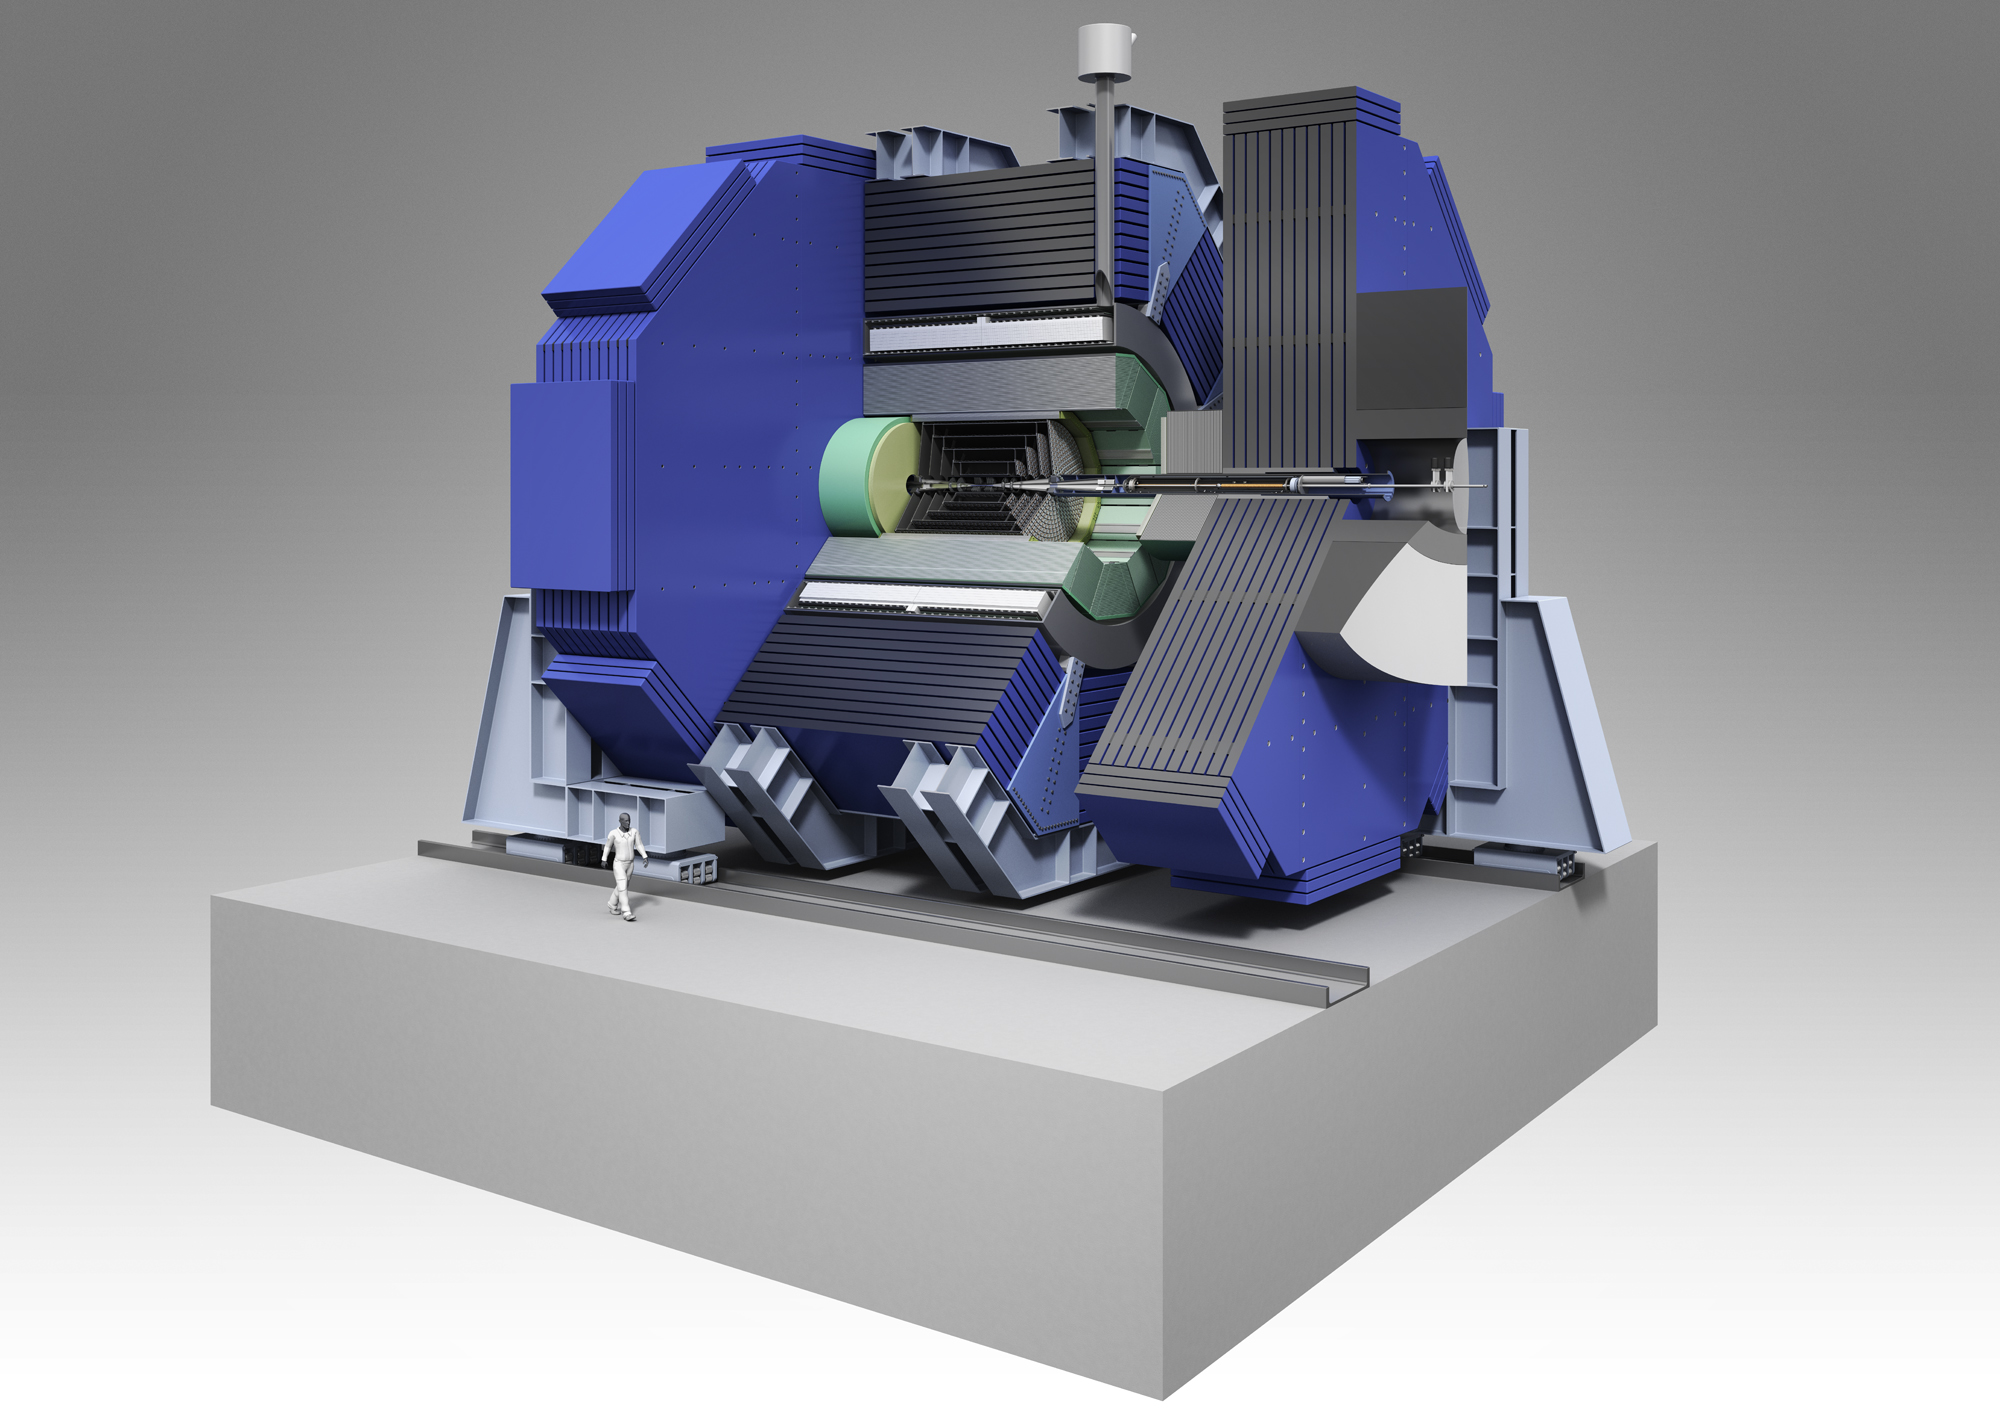
\includegraphics[width=0.5\textwidth]{figures/SiDmodel.jpg}
}
\end{center}
\end{column}

\begin{column}{0.48\textwidth}
\begin{center}
\visible<2->{\alert{ILD - International Large Detector}
\begin{itemize}
\item Height: $\sim$\SI{16}{\metre}, length:  $\sim$\SI{14}{\metre}
\item Weight: $\sim$\SI{14000}{\tonne}
\item Superconducting solenoid field: \SI{3.5}{\tesla}
\item TPC
\end{itemize}

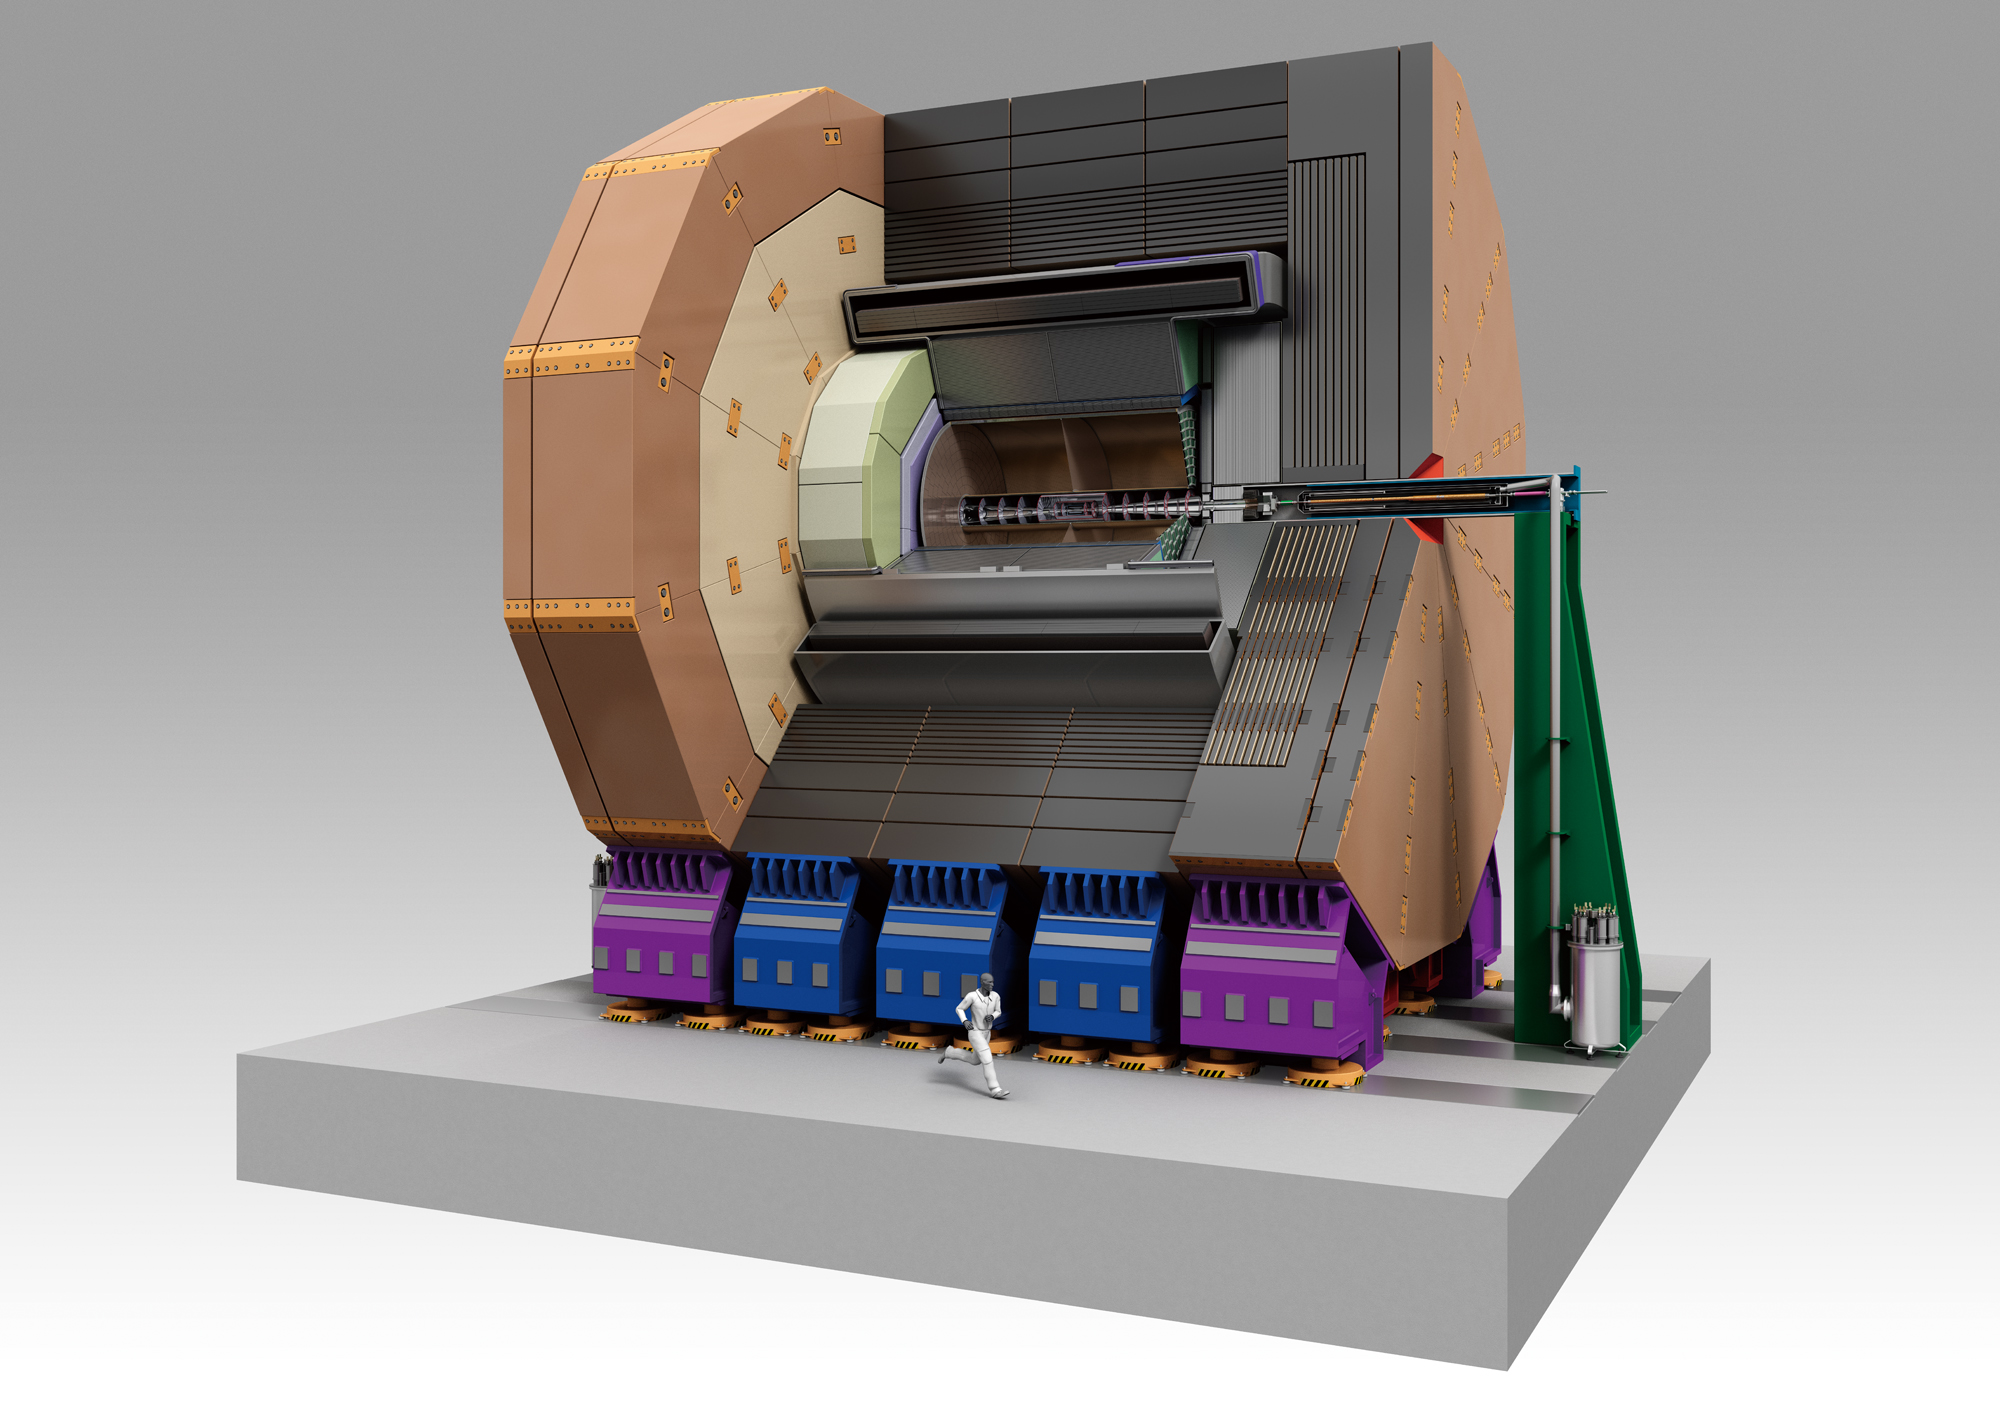
\includegraphics[width=0.5\textwidth]{figures/ILDmodel.jpg}
}
\end{center}
\end{column}
\end{columns}

\end{frame}
%--------------------------------------------------------------
\subsection{Physics motivation}
\begin{frame}[fragile]{The physics motivation of the ILC}
\ilclogo

\begin{block}{}
\centering
\textcolor{JungleGreen}{Cleanliness} - \textcolor{WildStrawberry}{Democracy} - \textcolor{Periwinkle}{Calculability} - \textcolor{LimeGreen}{Detail}
\end{block}

\visible<2->{
\begin{overprint}
\onslide<2>
\begin{itemize}
\color{JungleGreen}
\item Small background
\item Small detector occupancy
\item Smaller energy range
\item No out-of-time pileup or underlying events
\end{itemize}
\centering
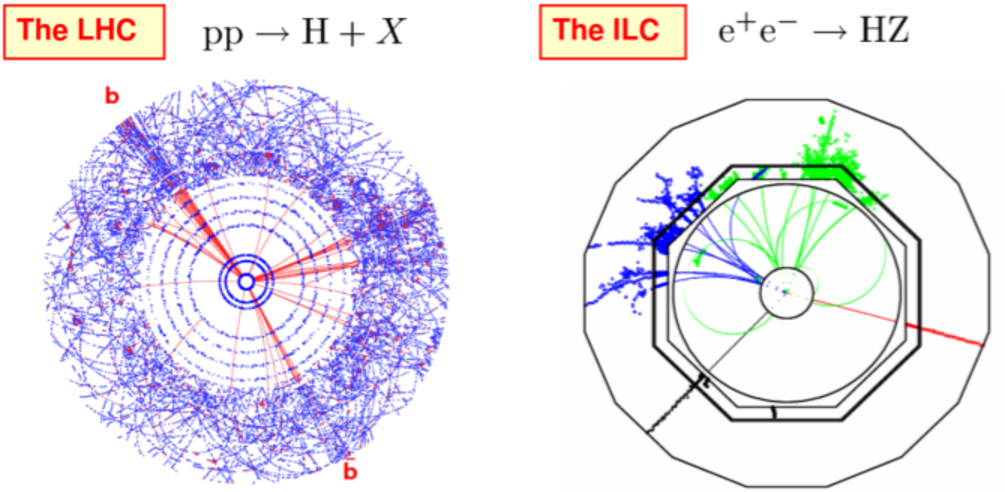
\includegraphics[width=0.6\textwidth]{figures/ILC_LHC_eventdisplay_comparison.pdf}

\onslide<3>
\begin{itemize}
\color{WildStrawberry}
\item Elementary coupling \textit{e} of photons is the same for all quarks and leptons
\item e$^+$e$^-$ annihilation produces pairs of all species, SM and exotics, at similar rates
\item No triggers
\end{itemize}

\onslide<4>
\begin{itemize}
\color{Periwinkle}
\item Point-like elementary particles in initial state
\item Coupling only to electroweak interactions
\item No systematic uncertainties due to PDF uncertainties and QCD corrections
\end{itemize}

\onslide<5>
\begin{itemize}
\color{LimeGreen}
\item Reconstruction of complete events
\item Quark and lepton momenta determined by kinematic fits
\item Study of spin-dependence of production and decay processes
\end{itemize}

\onslide<6>
\begin{columns}
\begin{column}{0.24\textwidth}
\begin{itemize}
\color{JungleGreen}
\item Small background
\item Small detector occupancy
\item Smaller energy range
\item No out-of-time pileup or underlying events
\end{itemize}
\end{column}
\begin{column}{0.26\textwidth}
\begin{itemize}
\color{WildStrawberry}
\item Elementary coupling \textit{e} of \textgamma \, the same for all quarks \& leptons
\item e$^+$e$^-$ annihilation produces pairs of all species, SM \& exotics, at similar rates
\item No triggers
\end{itemize}
\end{column}
\begin{column}{0.27\textwidth}
\begin{itemize}
\color{Periwinkle}
\item Pointlike elementary particles in initial state
\item Coupling only to EW interactions
\item No sys. uncert. due to PDF uncertainties and QCD corrections
\end{itemize}
\end{column}
\begin{column}{0.27\textwidth}
\begin{itemize}
\color{LimeGreen}
\item Reconstruction of complete events
\item Quark \& lepton momenta determined by kinematic fits
\item Study of spin-dependence of production \& decay process
\end{itemize}
\end{column}
\end{columns}
\end{overprint}
}%end visible
\end{frame}

\begin{frame}{The physics motivation of the ILC - Higgs factory}
\ilclogo
\begin{itemize}
\item Higgs factory\\
Fraction of the total cross section for Higgs production:\\
In pp: \num{e-9}, in e$^+$e$^-$: \num{e-2} $\approx$ 1\%
\item Each individual Higgs coupling will be measured to a percent accuracy, and the global width of the Higgs can be measured directly:\\LHC experiments have to make a global fit to all Higgs signals (plus using theoretical assumptions of the width), in order to get the Higgs couplings $ \rightarrow$ can never be as precise as at the ILC
\end{itemize}
\visible<2->{
\begin{columns}
 \begin{column}[t]{0.5\textwidth}
   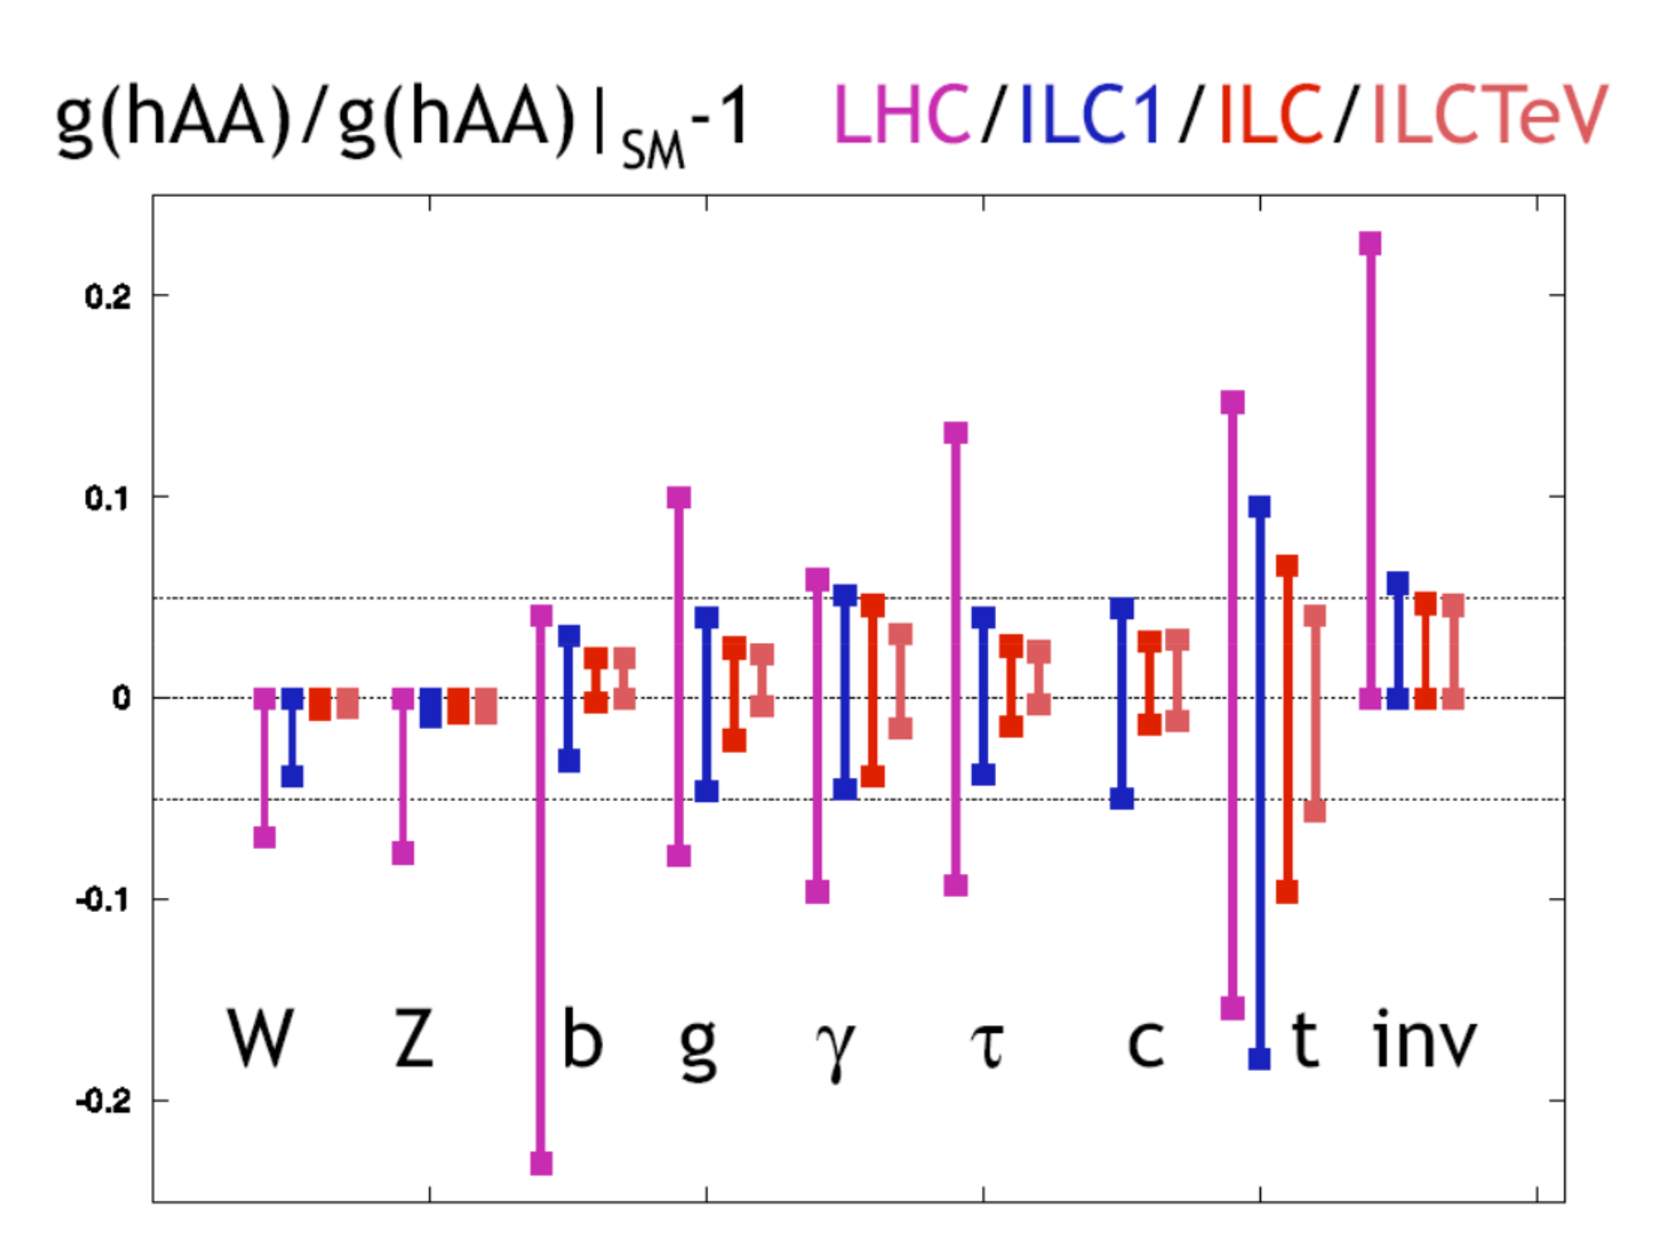
\includegraphics[width=0.85\textwidth]{figures/PhysicsMotivation-ILCPAC2012-Peskin_PrecisionHiggsCouplings.pdf}
 \end{column}
 \begin{column}[t]{0.5\textwidth}
   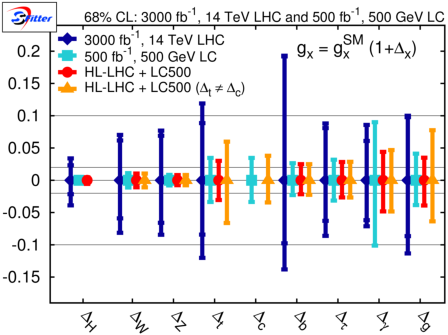
\includegraphics[width=0.83\textwidth]{figures/Higgs_Coupling_Precision_2013.pdf}
 \end{column}
\end{columns}
}
\end{frame}

\begin{frame}{The physics motivation of the ILC - Summary}
\ilclogo
\alert{\MakeUppercase{Precise measurements:}}\\
\begin{itemize}
\item The initial particle energy is precisely known. There are no PDFs, as the initial particles are elementary.
\item Due to the high energy resolution, peaks are now measurable that weren't measurable before. Particles with small mass difference are distinguishable.
\item c-tagging is possible because of small distance between IP and the  detectors (nano-sized beam)
\end{itemize}
\alert{\MakeUppercase{Clean environment:}}\\
\begin{itemize}
\item Due to polarization of both beams, background can be 'switched off'.
\item Small background and no underlying events or out-of-time pileup.
\end{itemize}
\alert{\MakeUppercase{Model independent:}}\\
\begin{itemize}
\item The reactions will be measured and reconstructed in completeness. No theoretical assumptions have to be taken into account.
\item New physics and BSM physics are accessible.
\end{itemize}

\end{frame}

\section{Background simulation and Final-Focus optimization}
\begin{frame}{Background simulation \& Final-Focus optimization}
\ilclogo
\begin{block}{}
\centering The ILC will be a \textcolor{Periwinkle}{high luminosity} particle accelerator \\with \textcolor{JungleGreen}{extraordinary precision}.
\end{block}
\vspace*{1cm}
\textcolor{JungleGreen}{The high precision depends on the cleanliness}, \textcolor{Periwinkle}{the high luminosity on the capability to focus the beam to nanometer size.}.\\
\vspace*{0.5cm}
\visible<2->{In order to minimize the effect of the background on the detectors and the measurements, the different background sources need to be modeled in great detail, \\also with respect to a possible optimization of the Final-Focus layout.}
\end{frame}

\subsection{SiD detector}
\begin{frame}{SiD detector}
\sidlogo
 I am in the SiD-Optimization group.\\
 Marcel Stanitzki is currently the SiD co-spokesperson.\\
 \vspace*{0.3cm}
 \visible<2->{
 \begin{columns}
  \begin{column}{0.7\textwidth}
    SiD has a very convincing design:
 \begin{itemize}
  \item compact and robust
  \item full silicon vertex detector and tracker\\
  Vertex detector:
  \begin{itemize}
   \item $<$\SI{5}{\micro\metre} resolution
   \item Momentum resolution $\sim$ 2-\SI{5e-5}{\per\giga\electronvolt}
   \item $\sim$ \SI{0.1}{\percent} X$_0$ per layer
    \item Single bunch timing resolution
    \item cos($\theta$)$\approx$0.984
  \end{itemize}
  \item highly granular calorimetry optimized for Particle Flow (ECAL: radation length = 26 X$_0$, \\EM energy resolution = 0.17/$\sqrt{E}\bigoplus$1\%)
 \end{itemize}
  \end{column}
  \begin{column}{0.3\textwidth}
    \begin{flushright}
  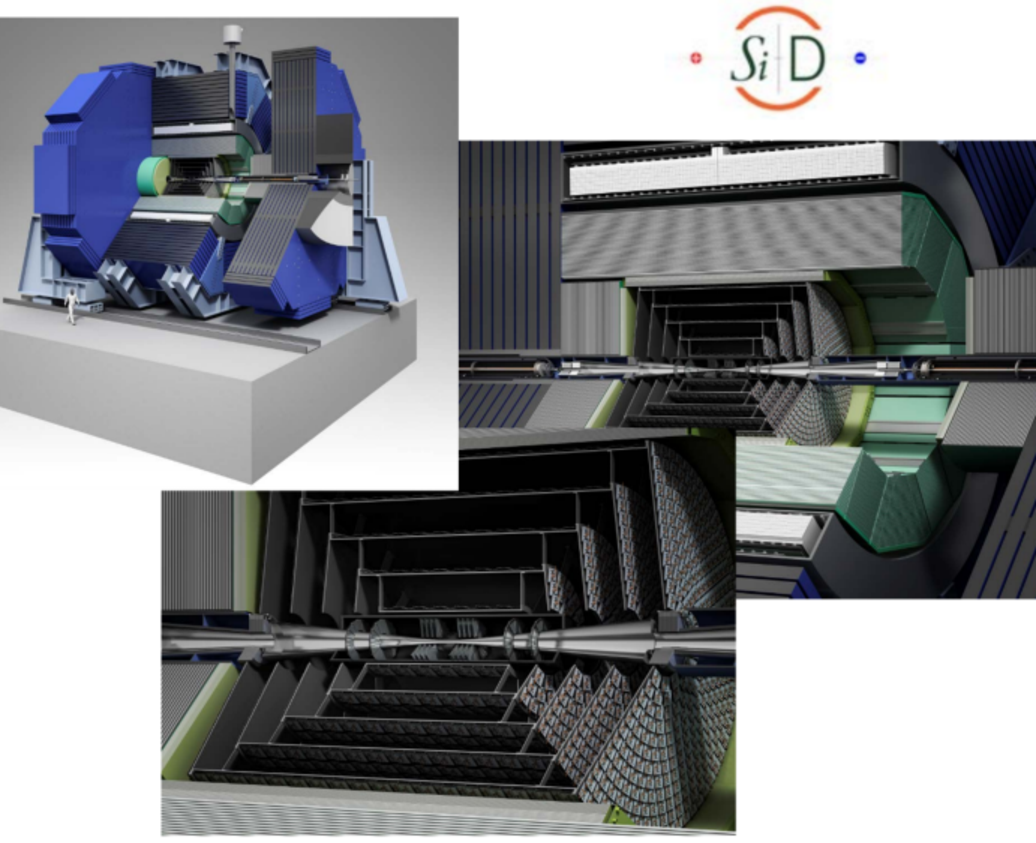
\includegraphics[height=0.4\textheight]{figures/SiDpics.pdf}
 \end{flushright}
  \end{column}
 \end{columns}
}
\end{frame}

\begin{frame}{SiD detector}
\sidlogo
\begin{figure}[T]
\centering
\begin{subfigure}[b]{0.49\textwidth}
\centering
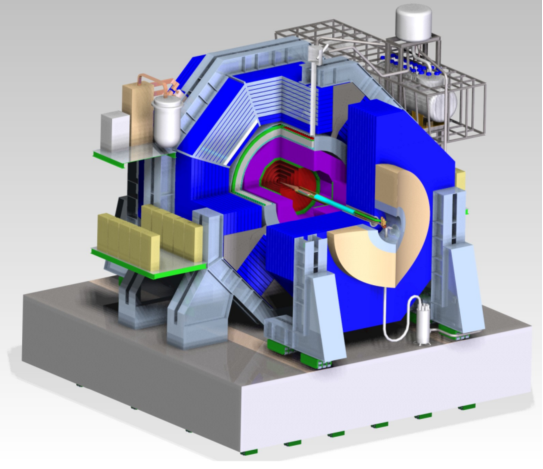
\includegraphics[height=0.65\textheight]{figures/SiD_detector_model.pdf}
\end{subfigure}
\begin{subfigure}[b]{0.49\textwidth}
\centering
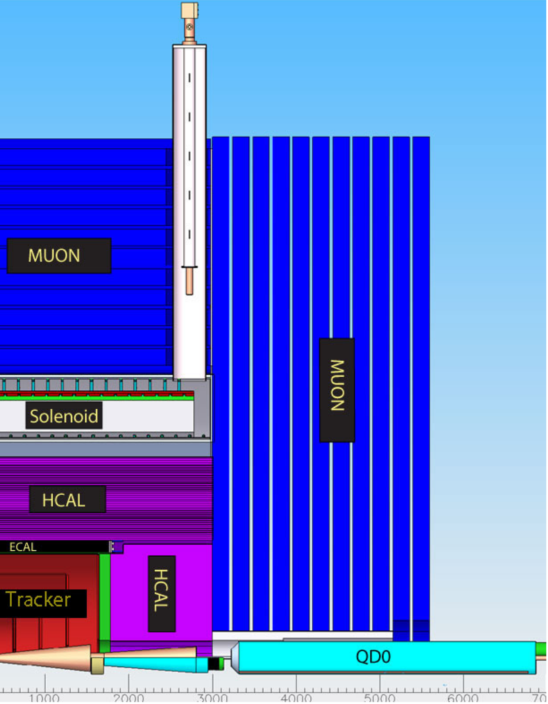
\includegraphics[height=0.65\textheight]{figures/SiD_detector_model_Ausschnitt.pdf}
\end{subfigure}
\caption{\small SiD detector model: Vertex detector (red), ECAL (green), HCAL (pink), Muon system (blue)}
\end{figure}
\end{frame}

\subsection{Background simulations}
\sidlogo
\begin{frame}{Simulation tools}
The background is first modeled in different simulation tools:\\
\begin{itemize}
\item \alert{GuineaPig} (Generator of background events from beam-beam interactions)
\item \alert{BDSIM} (Geant4 based extension toolkit for beam line simulations)
\item \alert{FLUKA} (Fully integrated particle physics MonteCarlo simulation package)
\end{itemize}
\vspace*{0.5cm}
The background events are then simulated in a \alert{full detector simulation} with a Geant4 toolkit.\\
\vspace*{0.2cm}
\begin{figure}
	\begin{columns}
        \column{0.7\linewidth} \flushright
        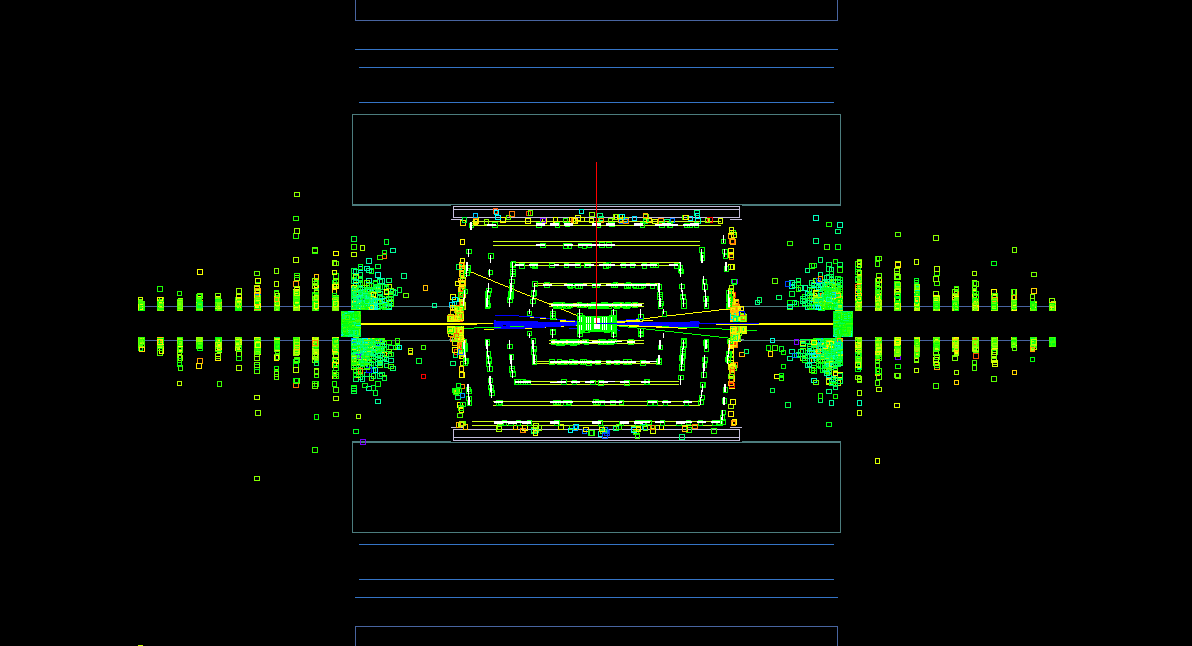
\includegraphics[width=0.61\textwidth]{figures/Full_bunchcrossing_rhoz.png}
        \column{0.3\linewidth}
        \caption{\small The inner detector part of SiD. WIRED4 event display of the pair background of one bunch crossing.}
      \end{columns}
\end{figure}
	
\end{frame}

\begin{frame}{Background sources}
\ilclogo
The main sources of background:
\begin{columns}
 \begin{column}{0.55\textwidth}
  \begin{itemize}
    \item Pair background
    \item Bhabha scattering
    \item \textgamma \textgamma $\rightarrow$ hadrons
    \item Neutrons from the beam dumps
    \item Background from Final-Focus system (beam halo collimators, muon spoilers)
  \end{itemize}
 \end{column}
 \begin{column}{0.45\textwidth}
 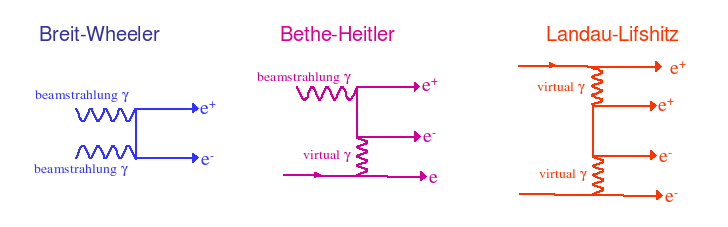
\includegraphics[height=0.2\textheight]{figures/beamstrahlung_processes.png}\\
 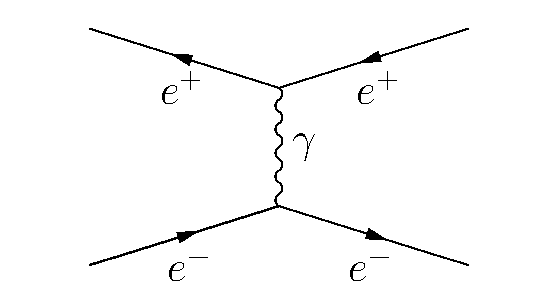
\includegraphics[height=0.15\textheight]{figures/bhabha_scattering.pdf} 
 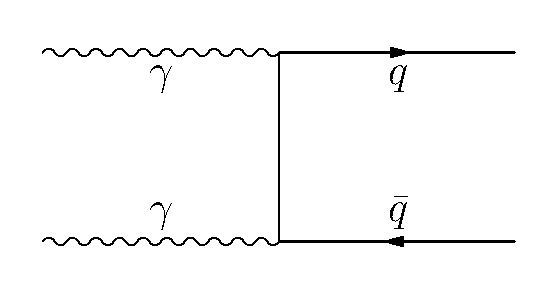
\includegraphics[height=0.15\textheight]{figures/gammagamma_hadrons.pdf}
 \end{column}
\end{columns}

\vspace*{0.5cm}
\visible<2->{
$\Rightarrow$So, if the ILC is supposed to see such clean signals, the question is:\\
\vspace*{0.5cm}
With all these background sources, how many background events do the detectors get?
}
\end{frame}

\begin{frame}{Pair background}
\sidlogo
 \begin{figure}
 	\begin{columns}
        \column[T]{0.75\linewidth} 
        \begin{flushright}
        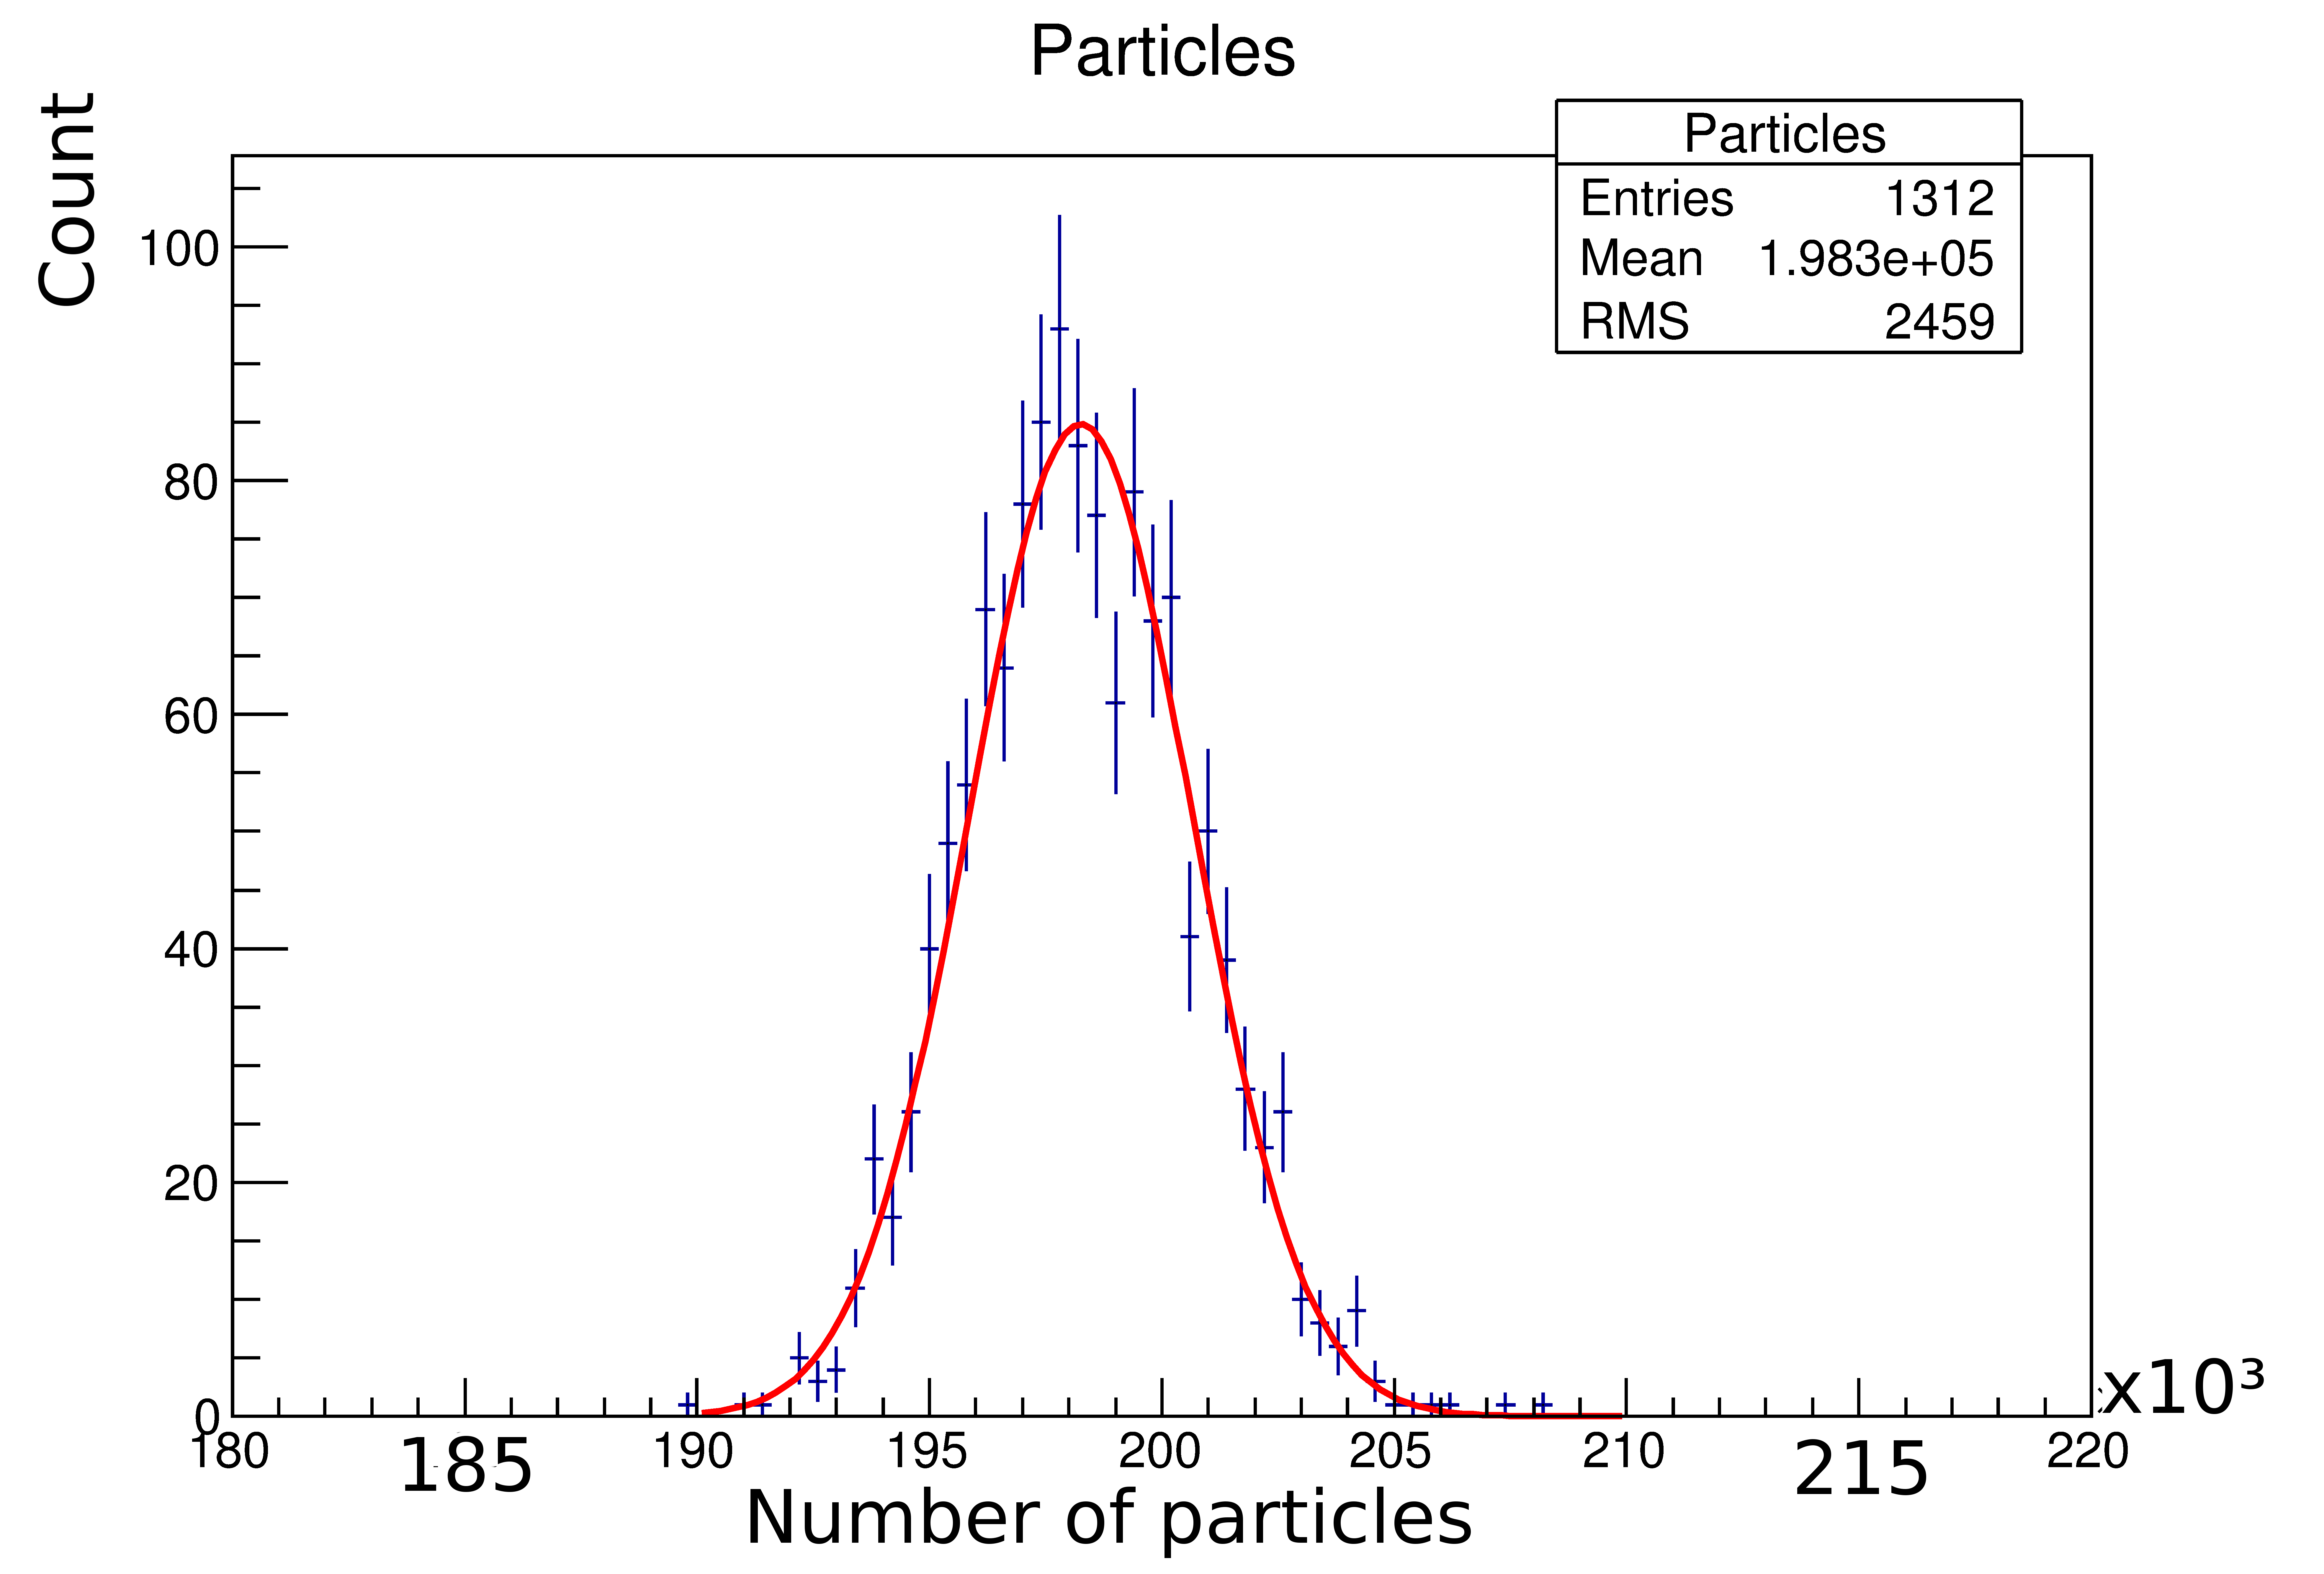
\includegraphics[height=0.55\textheight]{figures/sidloi3_pairs_1312_EcalEndcap_HitsPerFile_Particles.png}
        \end{flushright}
        \column[T]{0.25\linewidth}
        \begin{flushleft}
        \caption{\small Distribution of number of pair background particles per bunch crossing hitting the detector.}
        \end{flushleft}
      \end{columns}
\end{figure}
Per bunch, there are about \num{200000} pair background particles, in the whole detector.\\
\visible<2->{
\begin{center}
 In comparison:\\
e$^+$e$^-\rightarrow$\,W$^+$W$^-$ $\sim$ 1000/hour 
\hspace*{0.5cm}
e$^+$e$^-\rightarrow$\,HX $\sim$ 10/hour
\end{center}
}
\end{frame}


\begin{frame}{Hits in the SiD - EcalEndcaps}
\sidlogo
\begin{columns}
\begin{column}[T]{0.5\textwidth}
\begin{figure}
\centering
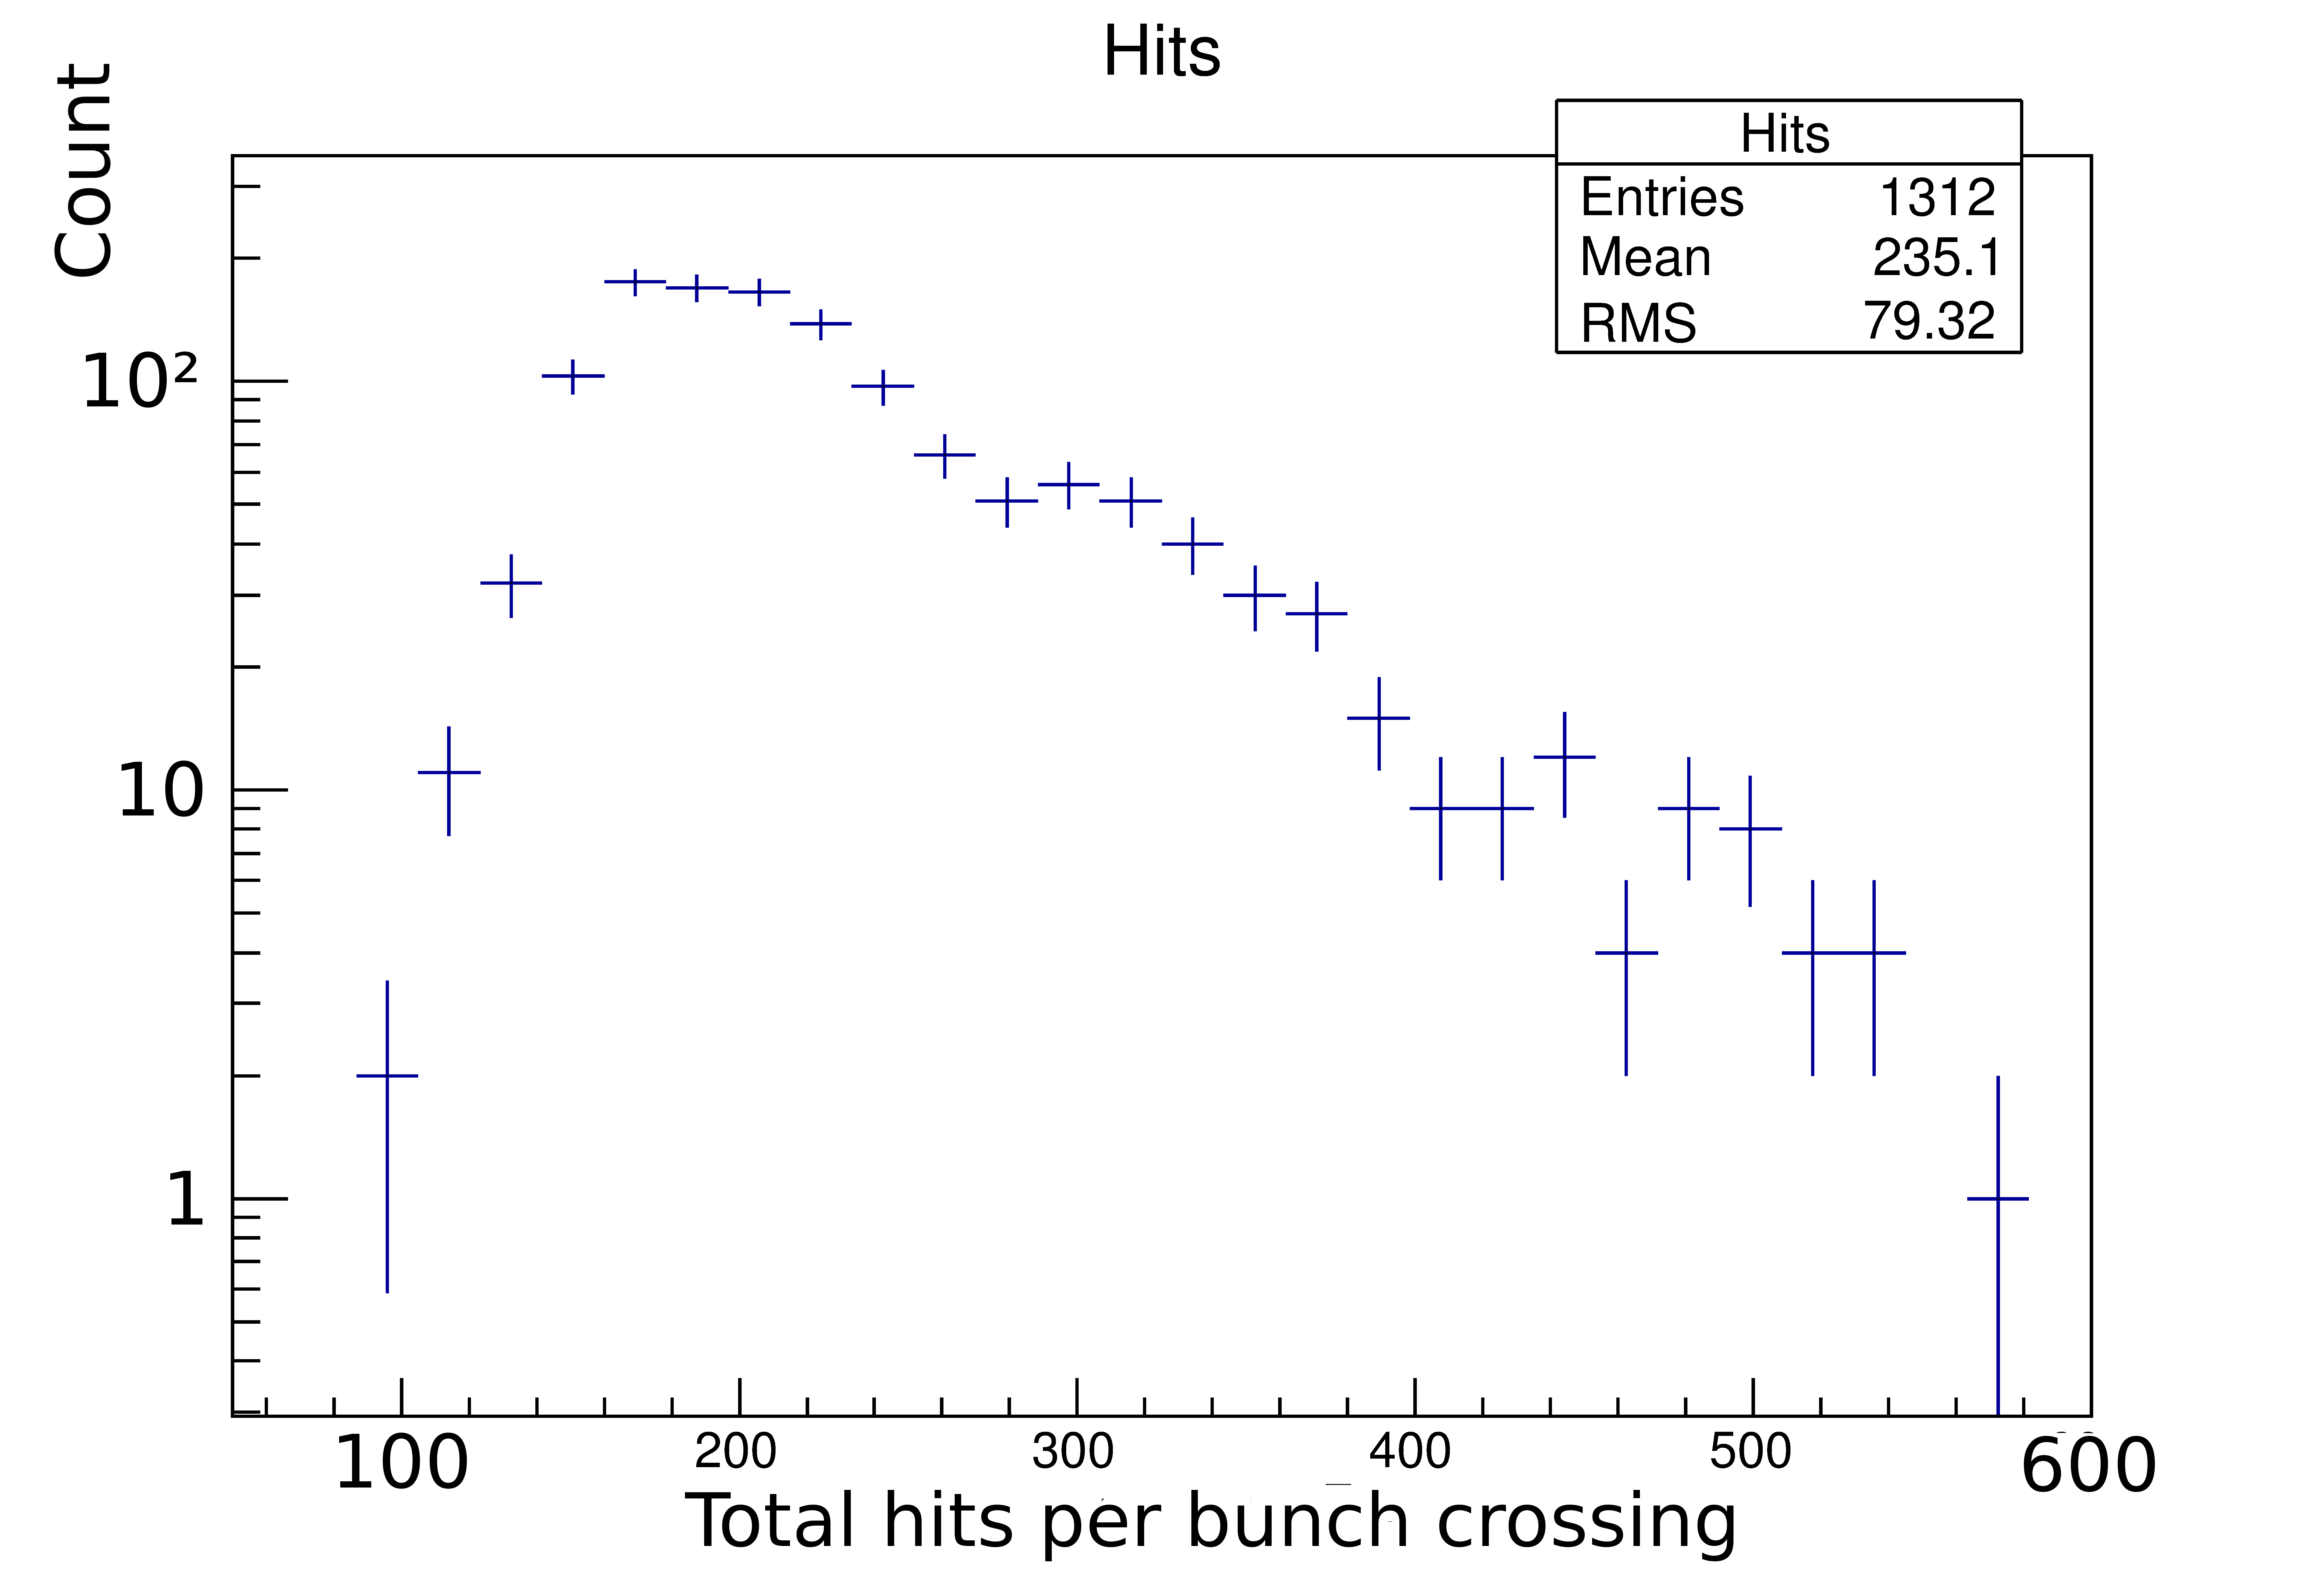
\includegraphics[width=\textwidth]{figures/sidloi3_pairs_1312_EcalEndcap_HitsPerFile_Hits.png}
\caption{\small Hits of pair background particles from a full train in the EcalEndcaps}
\end{figure}
\end{column}
\begin{column}[T]{0.5\textwidth}
\only<1>{
\begin{figure}
\centering
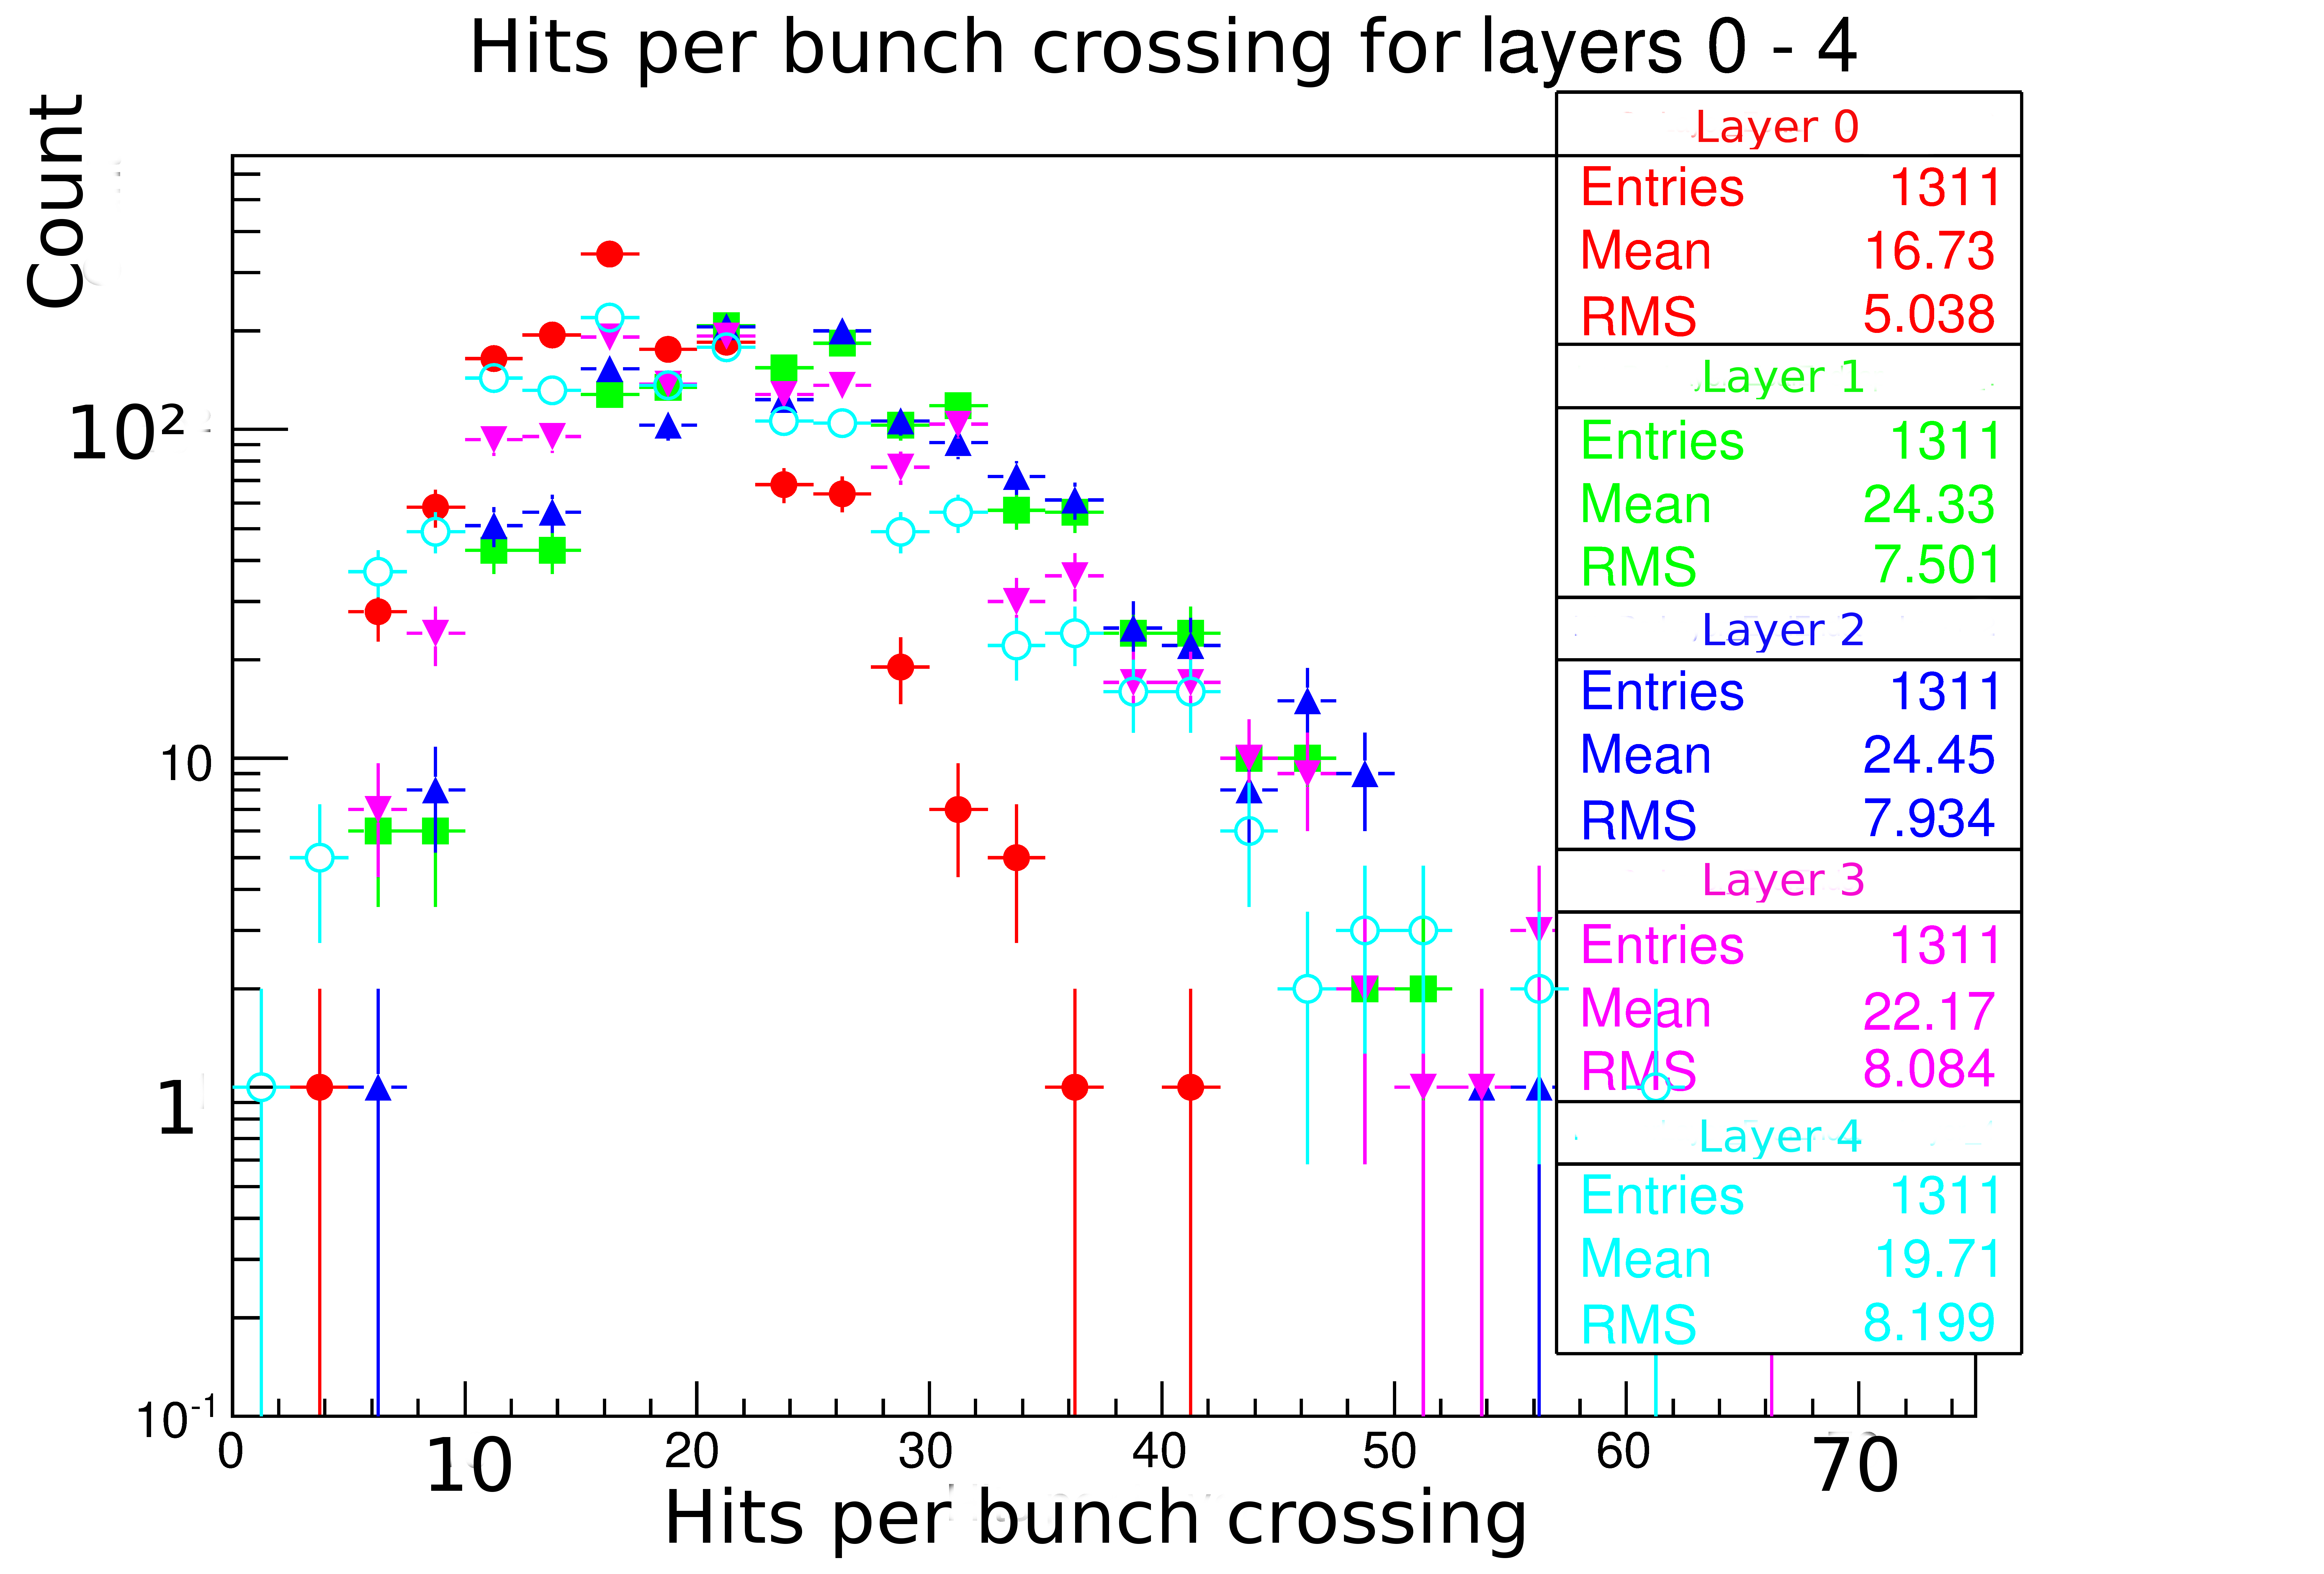
\includegraphics[width=\textwidth]{figures/sidloi3_pairs_1312_EcalEndcap_Hits_EcalEndcap_HitsPerLayer_EcalEndcap_Layer_0-4.png}
\caption{\small Comparison of the number of hits in the first 5 layers of the EcalEndcaps.}
\end{figure}
}
\only<2>{
\begin{figure}
\centering
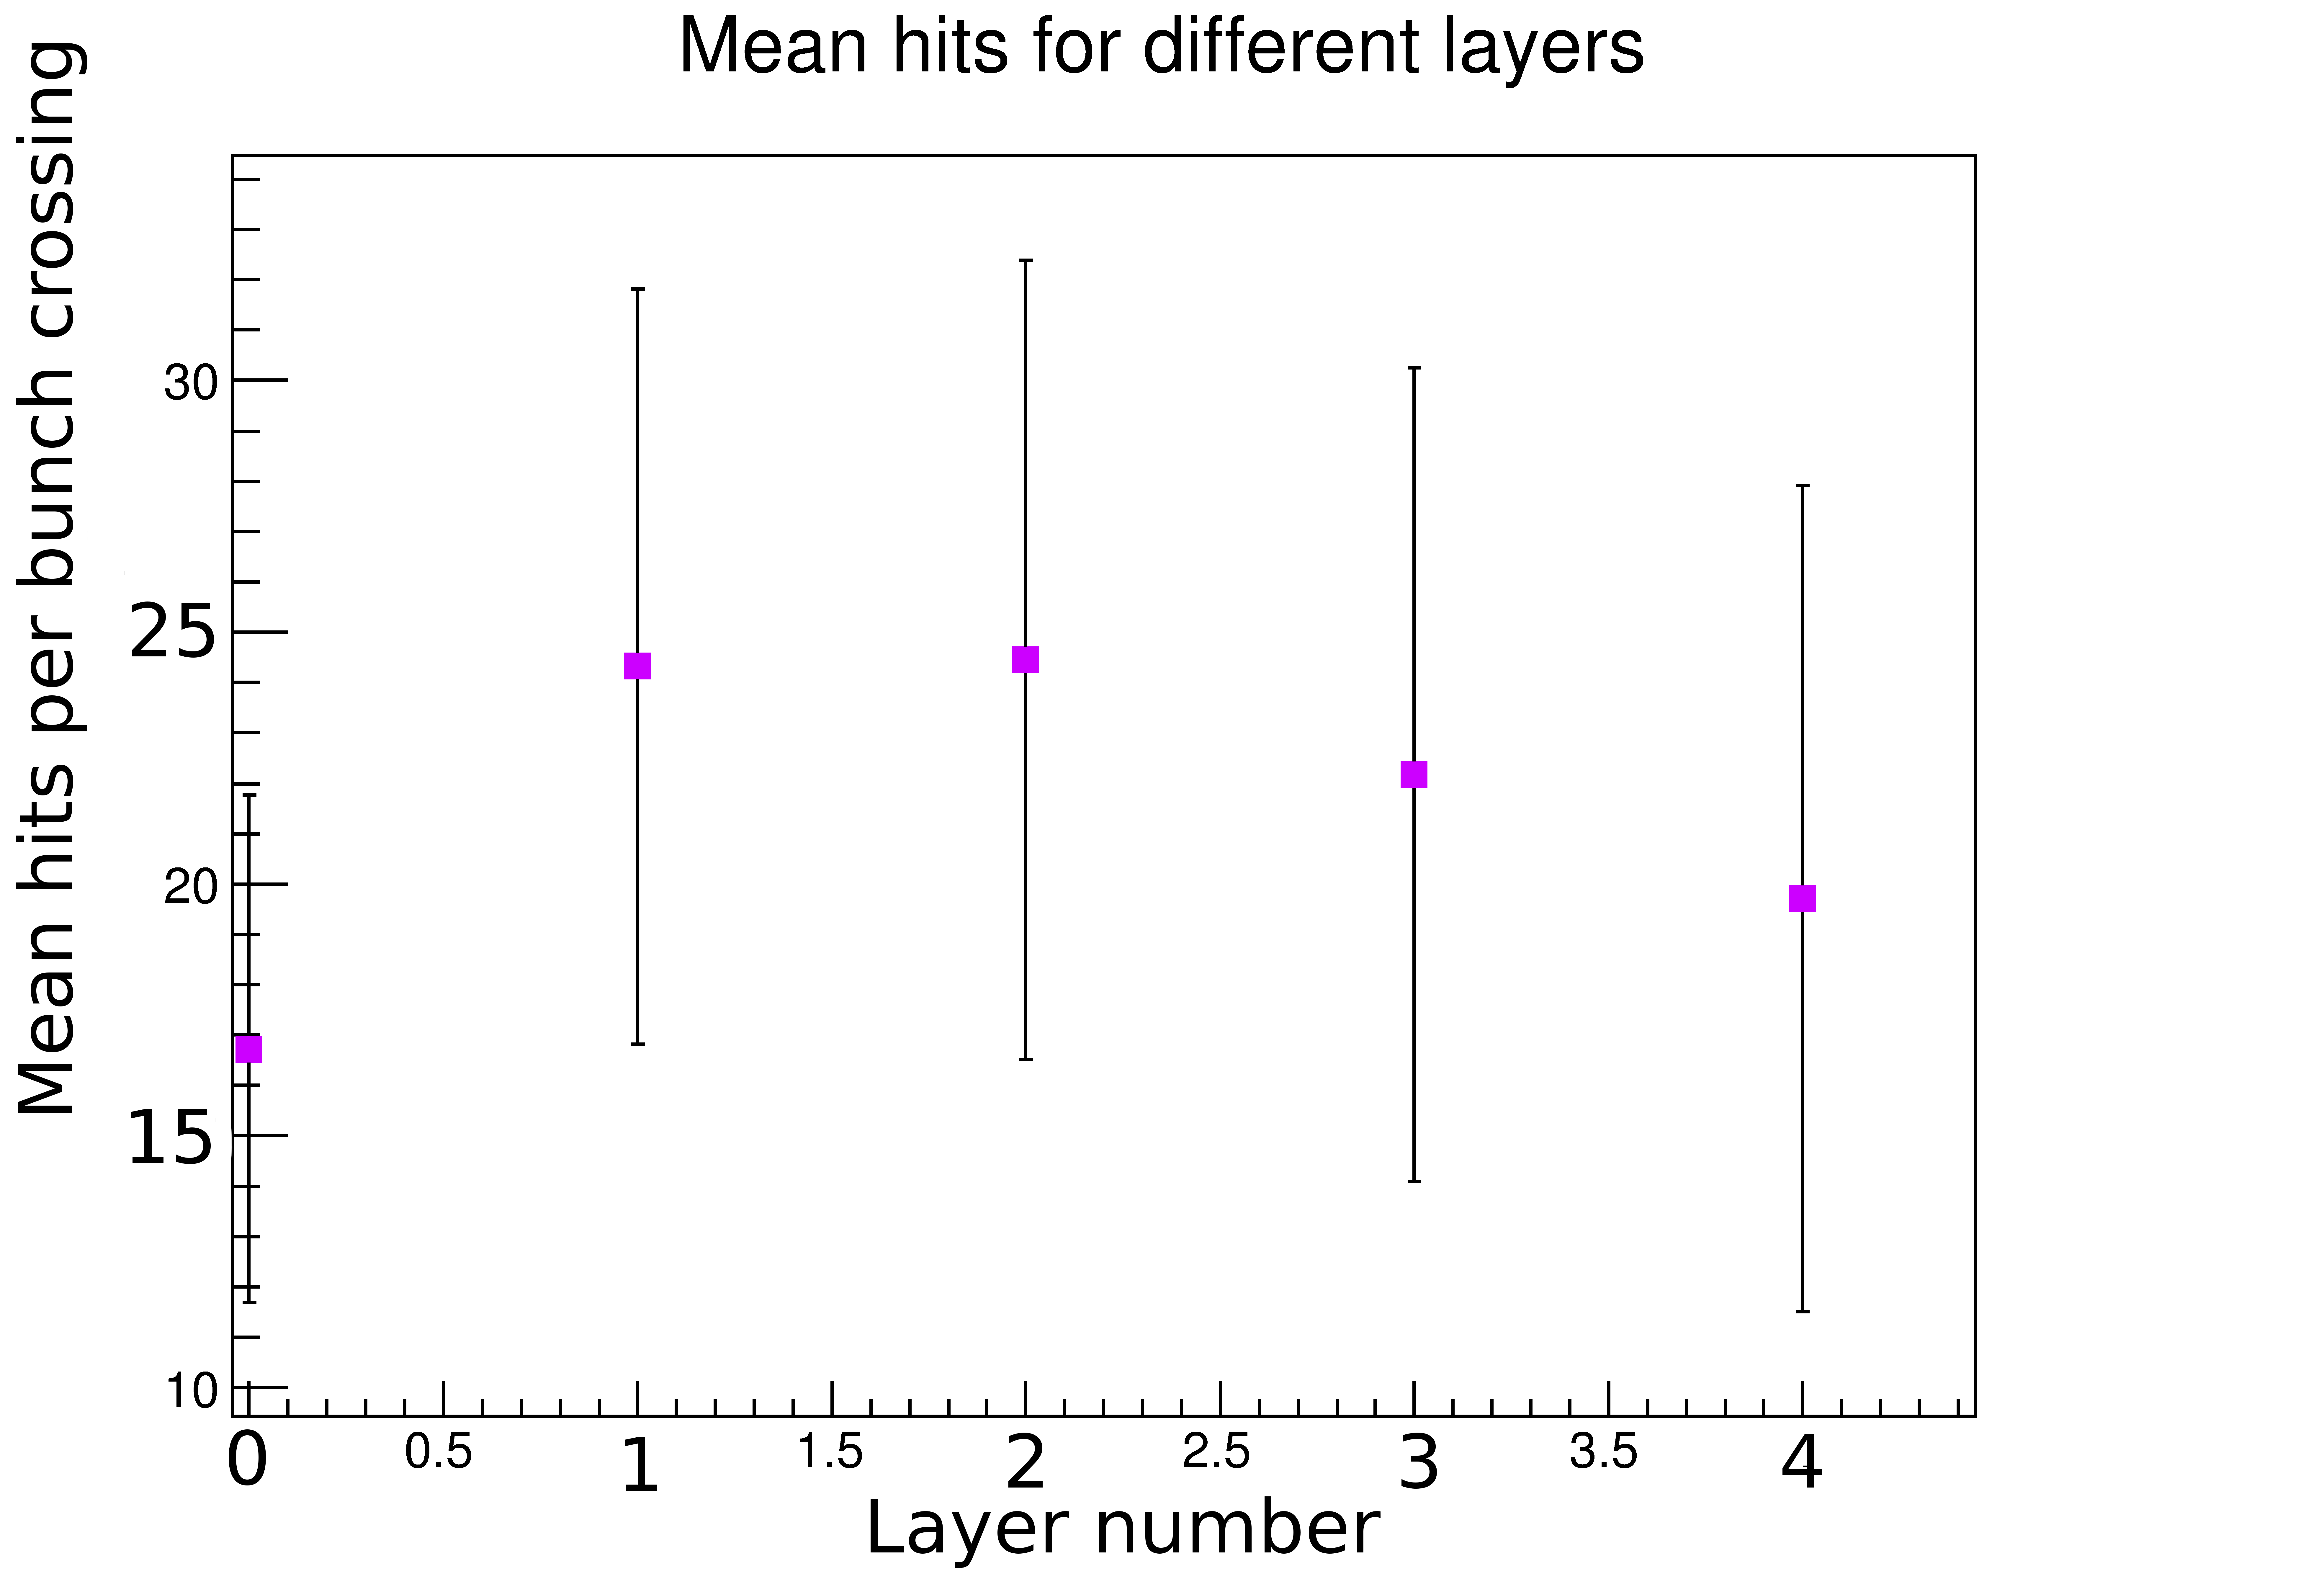
\includegraphics[width=\textwidth]{figures/sidloi3_pairs_1312_EcalEndcap_Hits_EcalEndcap_MeanHits_0-4.png}
\caption{\small Comparison of the MEAN number of hits in the first 5 layers of the EcalEndcaps.}
\end{figure}
}
\end{column}
\end{columns}
In the EcalEndcaps only, there are about 200 hits per bunch crossing.\\
The mean number of hits per layer is between 15 and 25 hits, per full bunch crossing!
\end{frame}

\begin{frame}{Hit maps of the inner most EcalEndcap layer}
\sidlogo
\begin{columns}[T]
\begin{column}[b]{0.5\textwidth}
 \begin{figure}
\centering
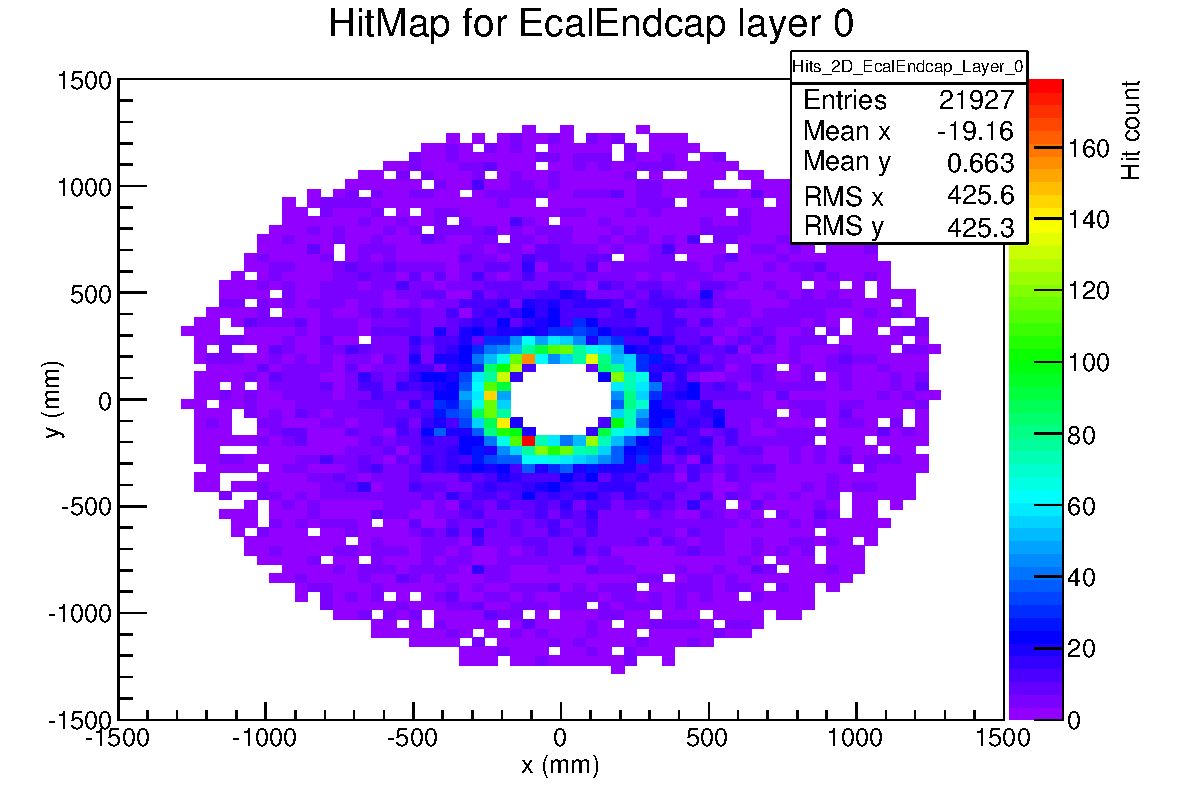
\includegraphics[height=0.5\textheight]{figures/sidloi3_pairs_1312_EcalEndcap_Hits_EcalEndcap_Hits_2D_EcalEndcap_Layer_0-eps-converted-to.pdf}
\caption{\small 2D hit map of the hits from a full pair background train in the EcalEndcap layer 0.}
\end{figure}
\end{column}
\begin{column}[b]{0.5\textwidth}
 \begin{figure}
\centering
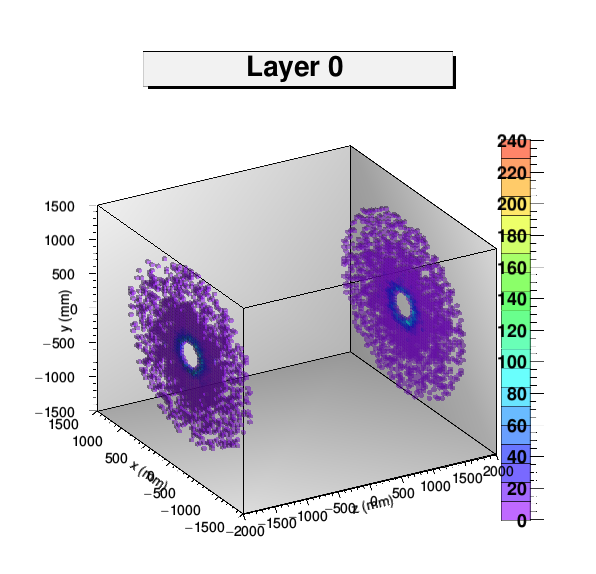
\includegraphics[height=0.5\textheight]{figures/Hits_3D_EcalEndcap_Layer_0.png}
\caption{\small 3D hit map of the hits from a full pair background train in the EcalEndcap layer 0.}
\end{figure}
\end{column}
\end{columns}
Most of the hits are around the beam pipe $\rightarrow$ Ring of fire
\end{frame}

\begin{frame}[t]{3D hit map animation of the EcalEndcaps}
\sidlogo
\begin{center}
  \animategraphics[portait,loop,height=7cm]{2}{3Danimation_EcalEndcap/Hits_3D_EcalEndcap_Layer_}{0}{30}
\end{center}
\end{frame}

\begin{frame}{Pair background origins}
\sidlogo
  \begin{figure}
 	\begin{columns}
        \column[T]{0.75\linewidth} 
        \begin{flushright}
        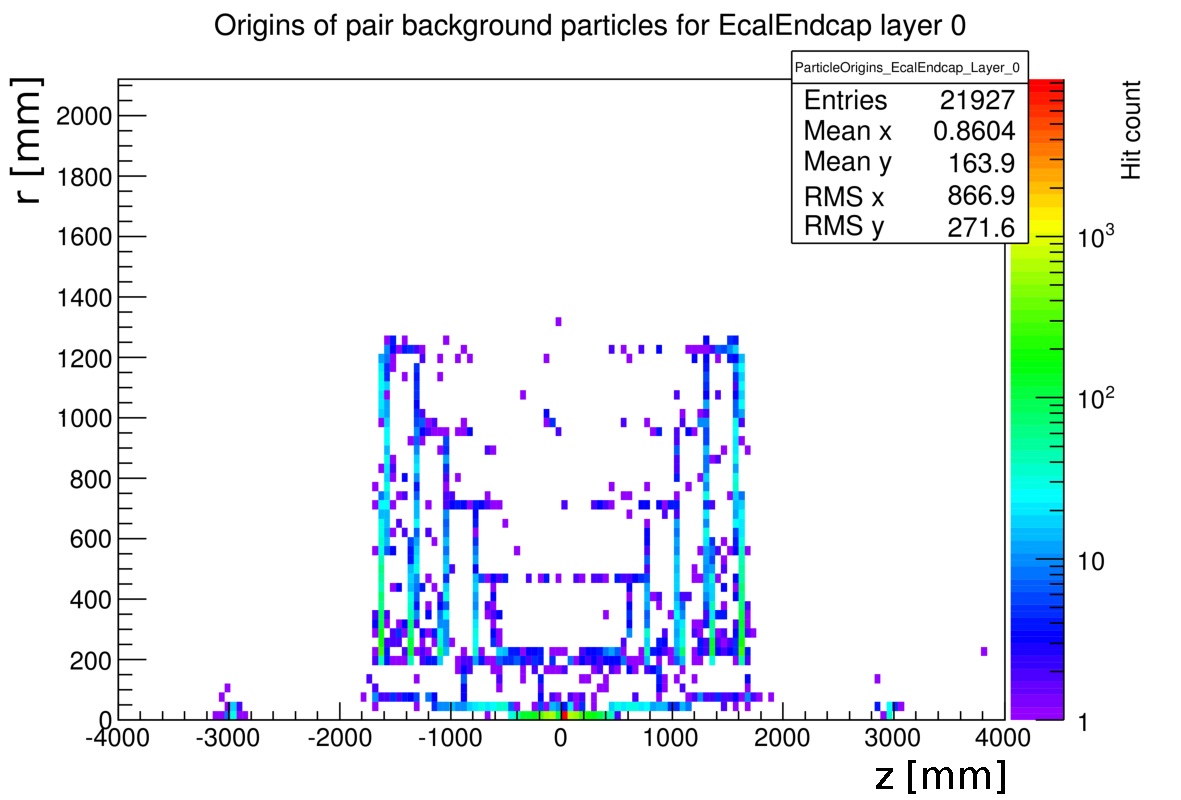
\includegraphics[width=0.9\textwidth]{figures/sidloi3_pairs_1312_EcalEndcap_Hits_EcalEndcap_ParticleOrigins_EcalEndcap_Layer_0.pdf}
        \end{flushright}
        \column[T]{0.25\linewidth}
        \begin{flushleft}
	\caption{\small 2D map of the origins of the pair background particles that hit the EcalEndcap layer 0.}
        \end{flushleft}
      \end{columns}
\end{figure}

Most of the background particles are coming from the IP as expected.\\
But there are a lot of particles backscattering from the tracker layers and the BeamCal.
\end{frame}


\begin{frame}{Absolute time of hits in the EcalEndcaps}
\sidlogo
\only<1>{
\begin{figure}
\centering
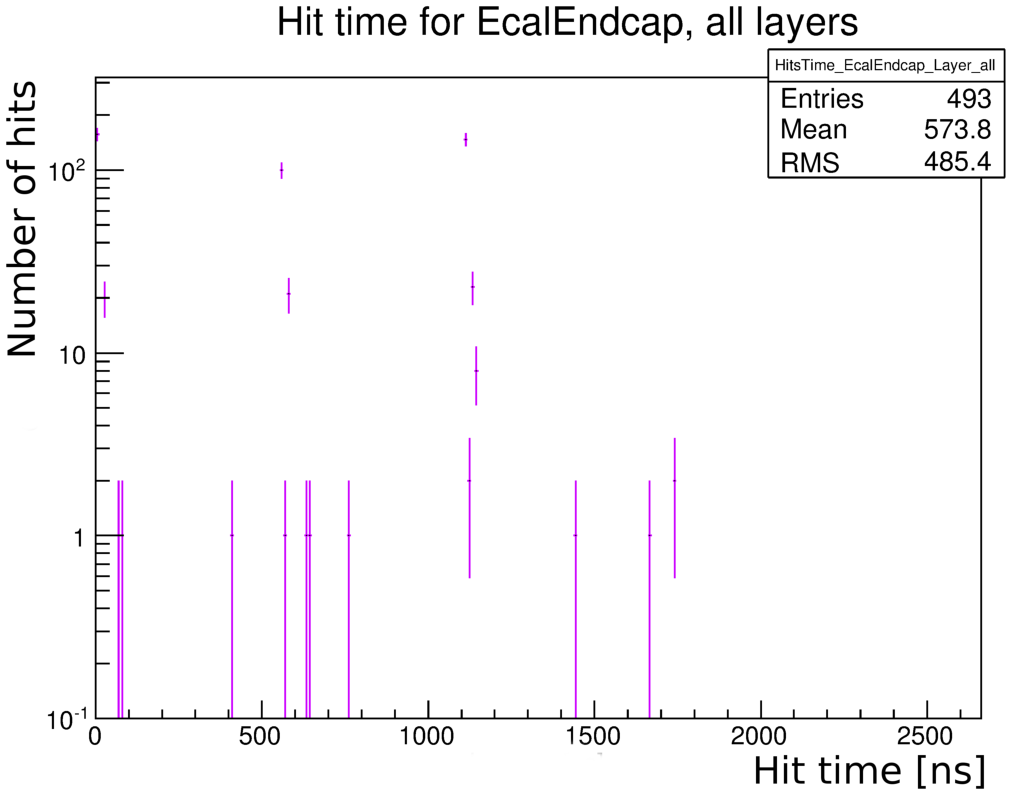
\includegraphics[height=0.55\textheight]{figures/3_sidloi3_EcalEndcap_Hits_EcalEndcap_HitsTime_EcalEndcap_Layer_all.pdf}
\caption{\small Number of particles arriving at the EcalEndcaps as a function of the absolute time.}
\end{figure}
}
\only<2>{
\begin{figure}
\centering
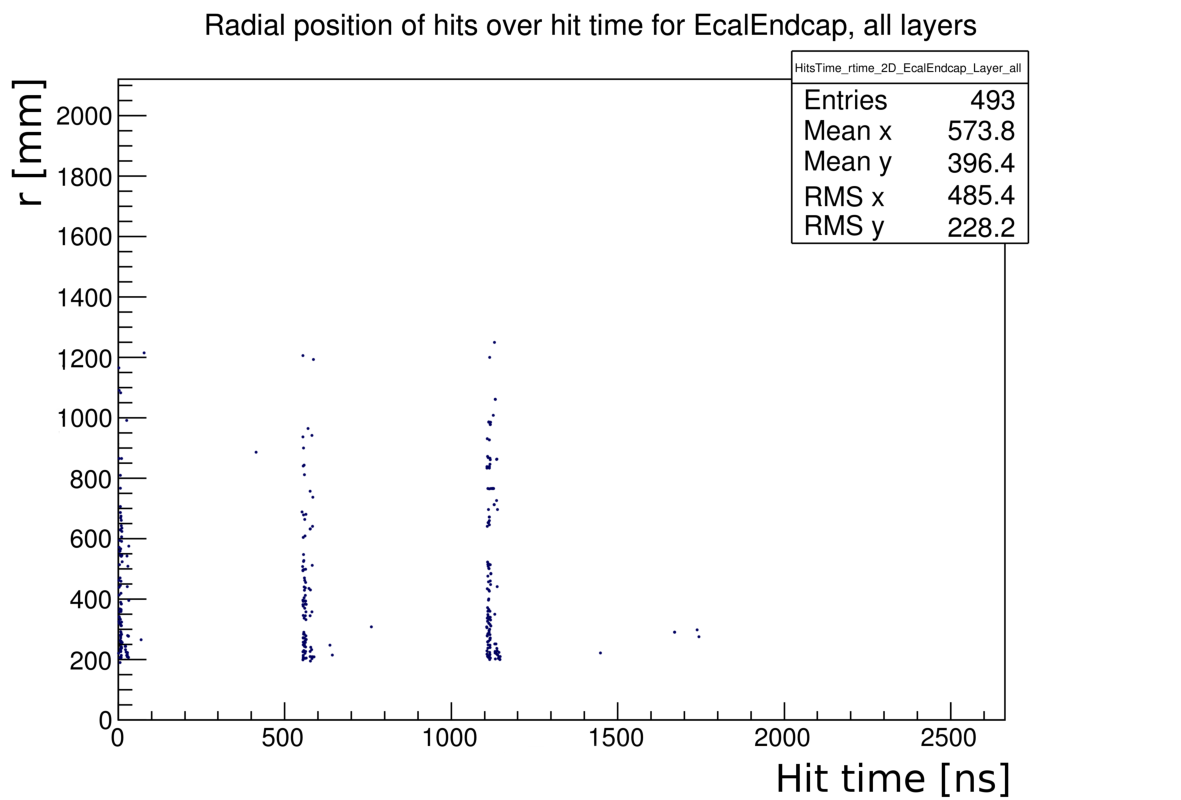
\includegraphics[height=0.6\textheight]{figures/3_sidloi3_EcalEndcap_Hits_EcalEndcap_HitsTime_rtime_2D_EcalEndcap_Layer_all-biggerdots.pdf}
\caption{\small The radial position of the particles arriving at the EcalEndcaps.}
\end{figure}
}
The pair background particles don't arrive all at the same time.\\
The second smaller peak of particles are backscatter particles.
\end{frame}

\begin{frame}{Interception}
\ilclogo
 \begin{center}
  There are many more really interesting and important things to study...\\
  \vspace*{1cm}
  \textit{How does the solenoid field affect the background?\\
  Do background particles backscatter more than once?\\
  With all background sources modeled, how many cell buffers will be filled - already only by the background?}
 \end{center}
 \vspace*{1cm}
  But I will tell you now about my next project!
\end{frame}


\subsection{ATF2}
\begin{frame}{Accelerator Test Facility 2}
ATF2
\begin{itemize}
\item Extension of the Accelerator Test Facility (ATF) at KEK in Japan
\item Test bench for the Final-Focus system of the ILC $\rightarrow$ very close to the ILC 500
\item Achieving \SI{42}{\nano\metre} beam size (goal: \SI{39}{\nano\metre})
\end{itemize}
\vspace*{0.3cm}
\begin{center}
 	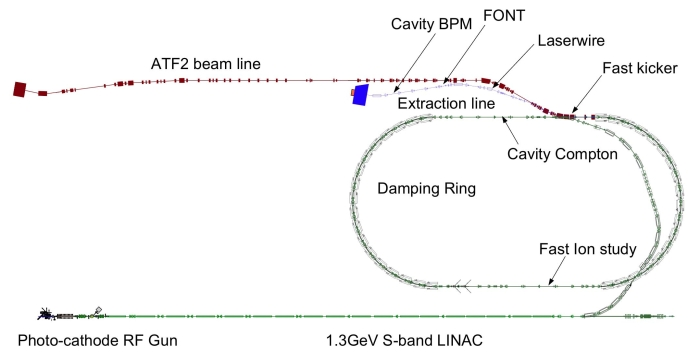
\includegraphics[width=0.8\textwidth]{figures/ATF.jpg}
\end{center}

\end{frame}

\begin{frame}{Beam time in March}
\ejadelogo
As the E-JADE program {\tiny(www.e-jade.eu)} is funding a two months trip to Japan for me,
I will be able to join the beam time at ATF2 in March:
\begin{itemize}
\item Operating the ATF beam
\item Installing a new beam halo collimator
\item Measuring the beam size and the beam halo
\item Wakefield measurements
\item Studies of the generated background with Cherenkov detectors
\end{itemize}
%\vspace*{0.5cm}
\begin{center}
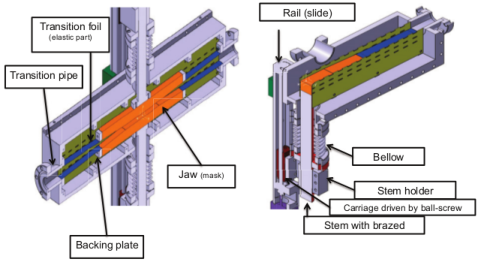
\includegraphics[width=0.65\textwidth]{figures/ATF2_beamhalo_collimator.pdf}
\end{center}

\end{frame}

\section*{The end}
{
\usebackgroundtemplate{
 \tikz\node[opacity=0.1]{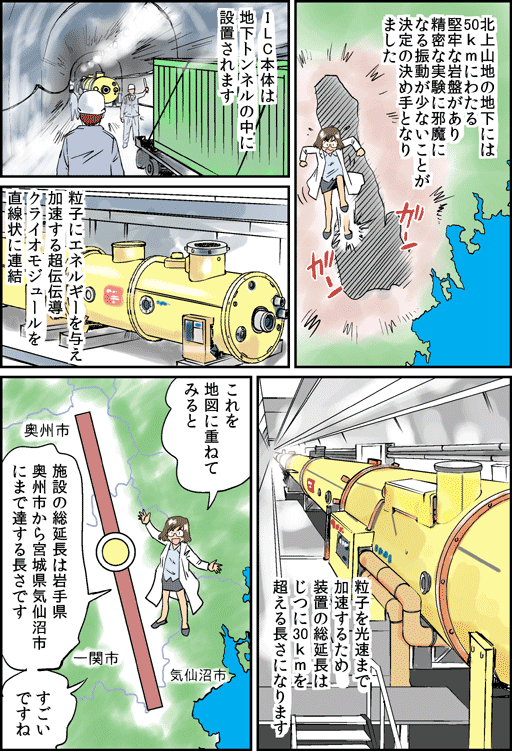
\includegraphics[width=\paperwidth,resolution=200]{figures/ilc-Comic.png}};
 % \tikz\node[opacity=0.2]{\centering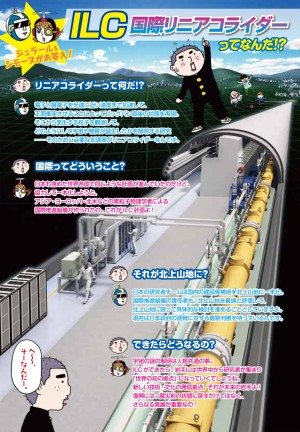
\includegraphics[height=\paperheight]{figures/Iwatecomics.jpg}};
 }
\begin{frame}
\ilclogo
\begin{center}
 If you are now interested in SiD and keen on working for the ILC, \\
if you like working in a very international environment, \\
or if you love Japan,\\
there are lots of possible Master's and Ph.D topics.\\
\vspace*{1cm}
\textcolor{RubineRed}{
	\LARGE Thanks!\\
	\begin{CJK}{UTF8}{min}
	どうもありがとうございます。
	\end{CJK}
}
\end{center}
\end{frame}
}

\section*{References}
\begin{thebibliography}{9}
\begin{frame}{References}
\bibitem{TDR} T. Behnke, et al.
\emph{The International Linear Collider - Technical Design Report}, 2013.
\bibitem{LHC TDR} \emph{LHC - Design Report}, \url{http://ab-div.web.cern.ch/ab-div/Publications/LHC-DesignReport.html}
\bibitem{IP beam parameters} ATLAS-CONF-2010-027. \emph{Characterization of Interaction-Point Beam Parameters Using the pp Event-Vertex Distribution Reconstructed in the ATLAS Detector at the LHC}, 2010. \url{http://cds.cern.ch/record/1277659/files/ATLAS-CONF-2010-027.pdf}
\bibitem{ILCPAC2012} M. Peskin. \emph{Physics Motivation for the ILC}, 2012. \url{http://www.fnal.gov/directorate/ILCPAC/2012Dec/Physics-ILCPAC2012-Peskin.pdf}
\end{frame}
\begin{frame}{References}
\bibitem{MIT2013} Klute, Markus, Rémi Lafaye, Tilman Plehn, Michael Rauch, and
Dirk Zerwas. \emph{Measuring Higgs Couplings at a Linear Collider}
EPL (Europhysics Letters) 101, no. 5 (March 1, 2013): 51001. \url{http://dx.doi.org/10.1209/0295-5075/101/51001}
\bibitem{RHUL} Mark Thomson. \emph{Physics and Detectors at the ILC}, 2013. \url{https://www.royalholloway.ac.uk/physics/documents/pdf/events/particlephysicsseminars/13-14markthomson23oct2013.pdf}
\bibitem{ATF2} Kuroda et al. \emph{A plan of KEK-ATF Final Focus Test Beam Line (ATF2)
}. \url{http://icfa-nanobeam.web.cern.ch/icfa-nanobeam/paper/urakawa_ATF2-2.pdf}

\end{frame}
\end{thebibliography}

%--------------------------------------------------------------------------------
\appendix

\begin{frame}
\begin{center}
\LARGE Additional Material
\end{center}
  \tableofcontents
\end{frame}

\section{ILC parameters}
\begin{frame}{ILC baseline parameters}
\ilclogo
\centering
	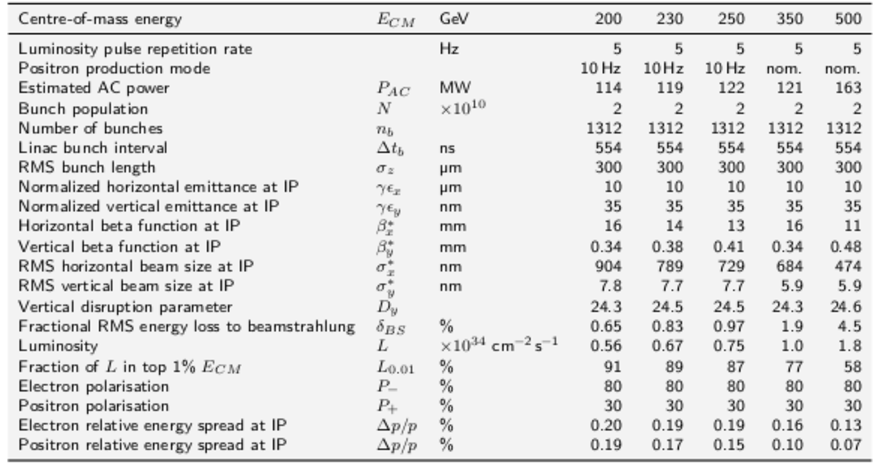
\includegraphics[width=\textwidth]{figures/ILCTDR-VOLUME_3-PART_II_ILCparameters.pdf}
\end{frame}
\begin{frame}{ILC parameters for the different upgrade stages}
\ilclogo
\centering
	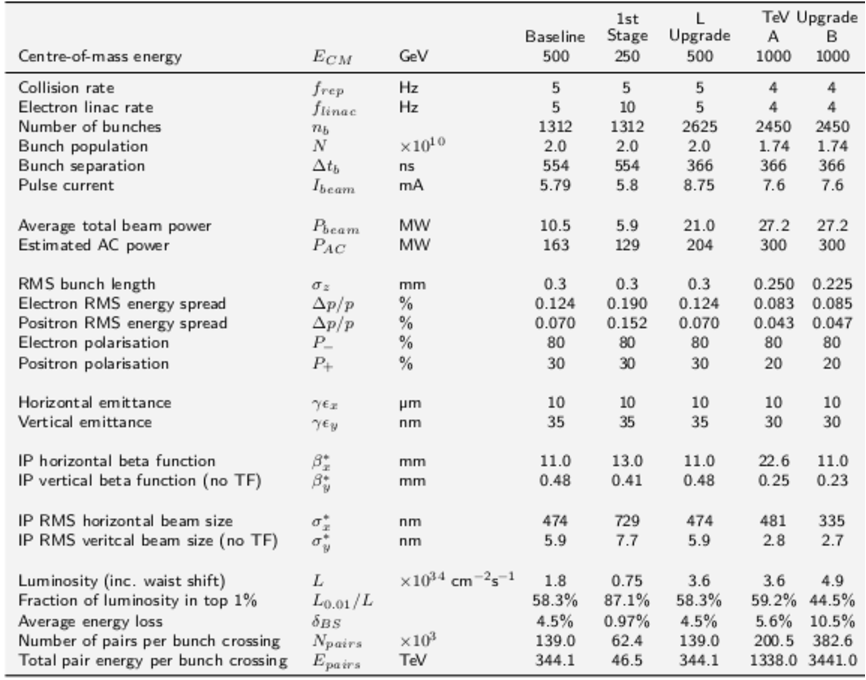
\includegraphics[width=0.8\textwidth]{figures/ILCTDR-VOLUME_3-PART_II_ILCparametersUpgrades.pdf}
\end{frame}

\section{Basic accelerating structure}
\begin{frame}{Basic accelerating structure}
\ilclogo
The main accelerating structures are the two 11km long LINACs.
\begin{itemize}
\item 9-cell superconducting RF cavities operating at 1.3 GHz 
\item Accelerating gradient of >30 MV/m
\item Electrons and positrons accelerated in RF standing waves in the cavities 
\end{itemize}
\begin{center}
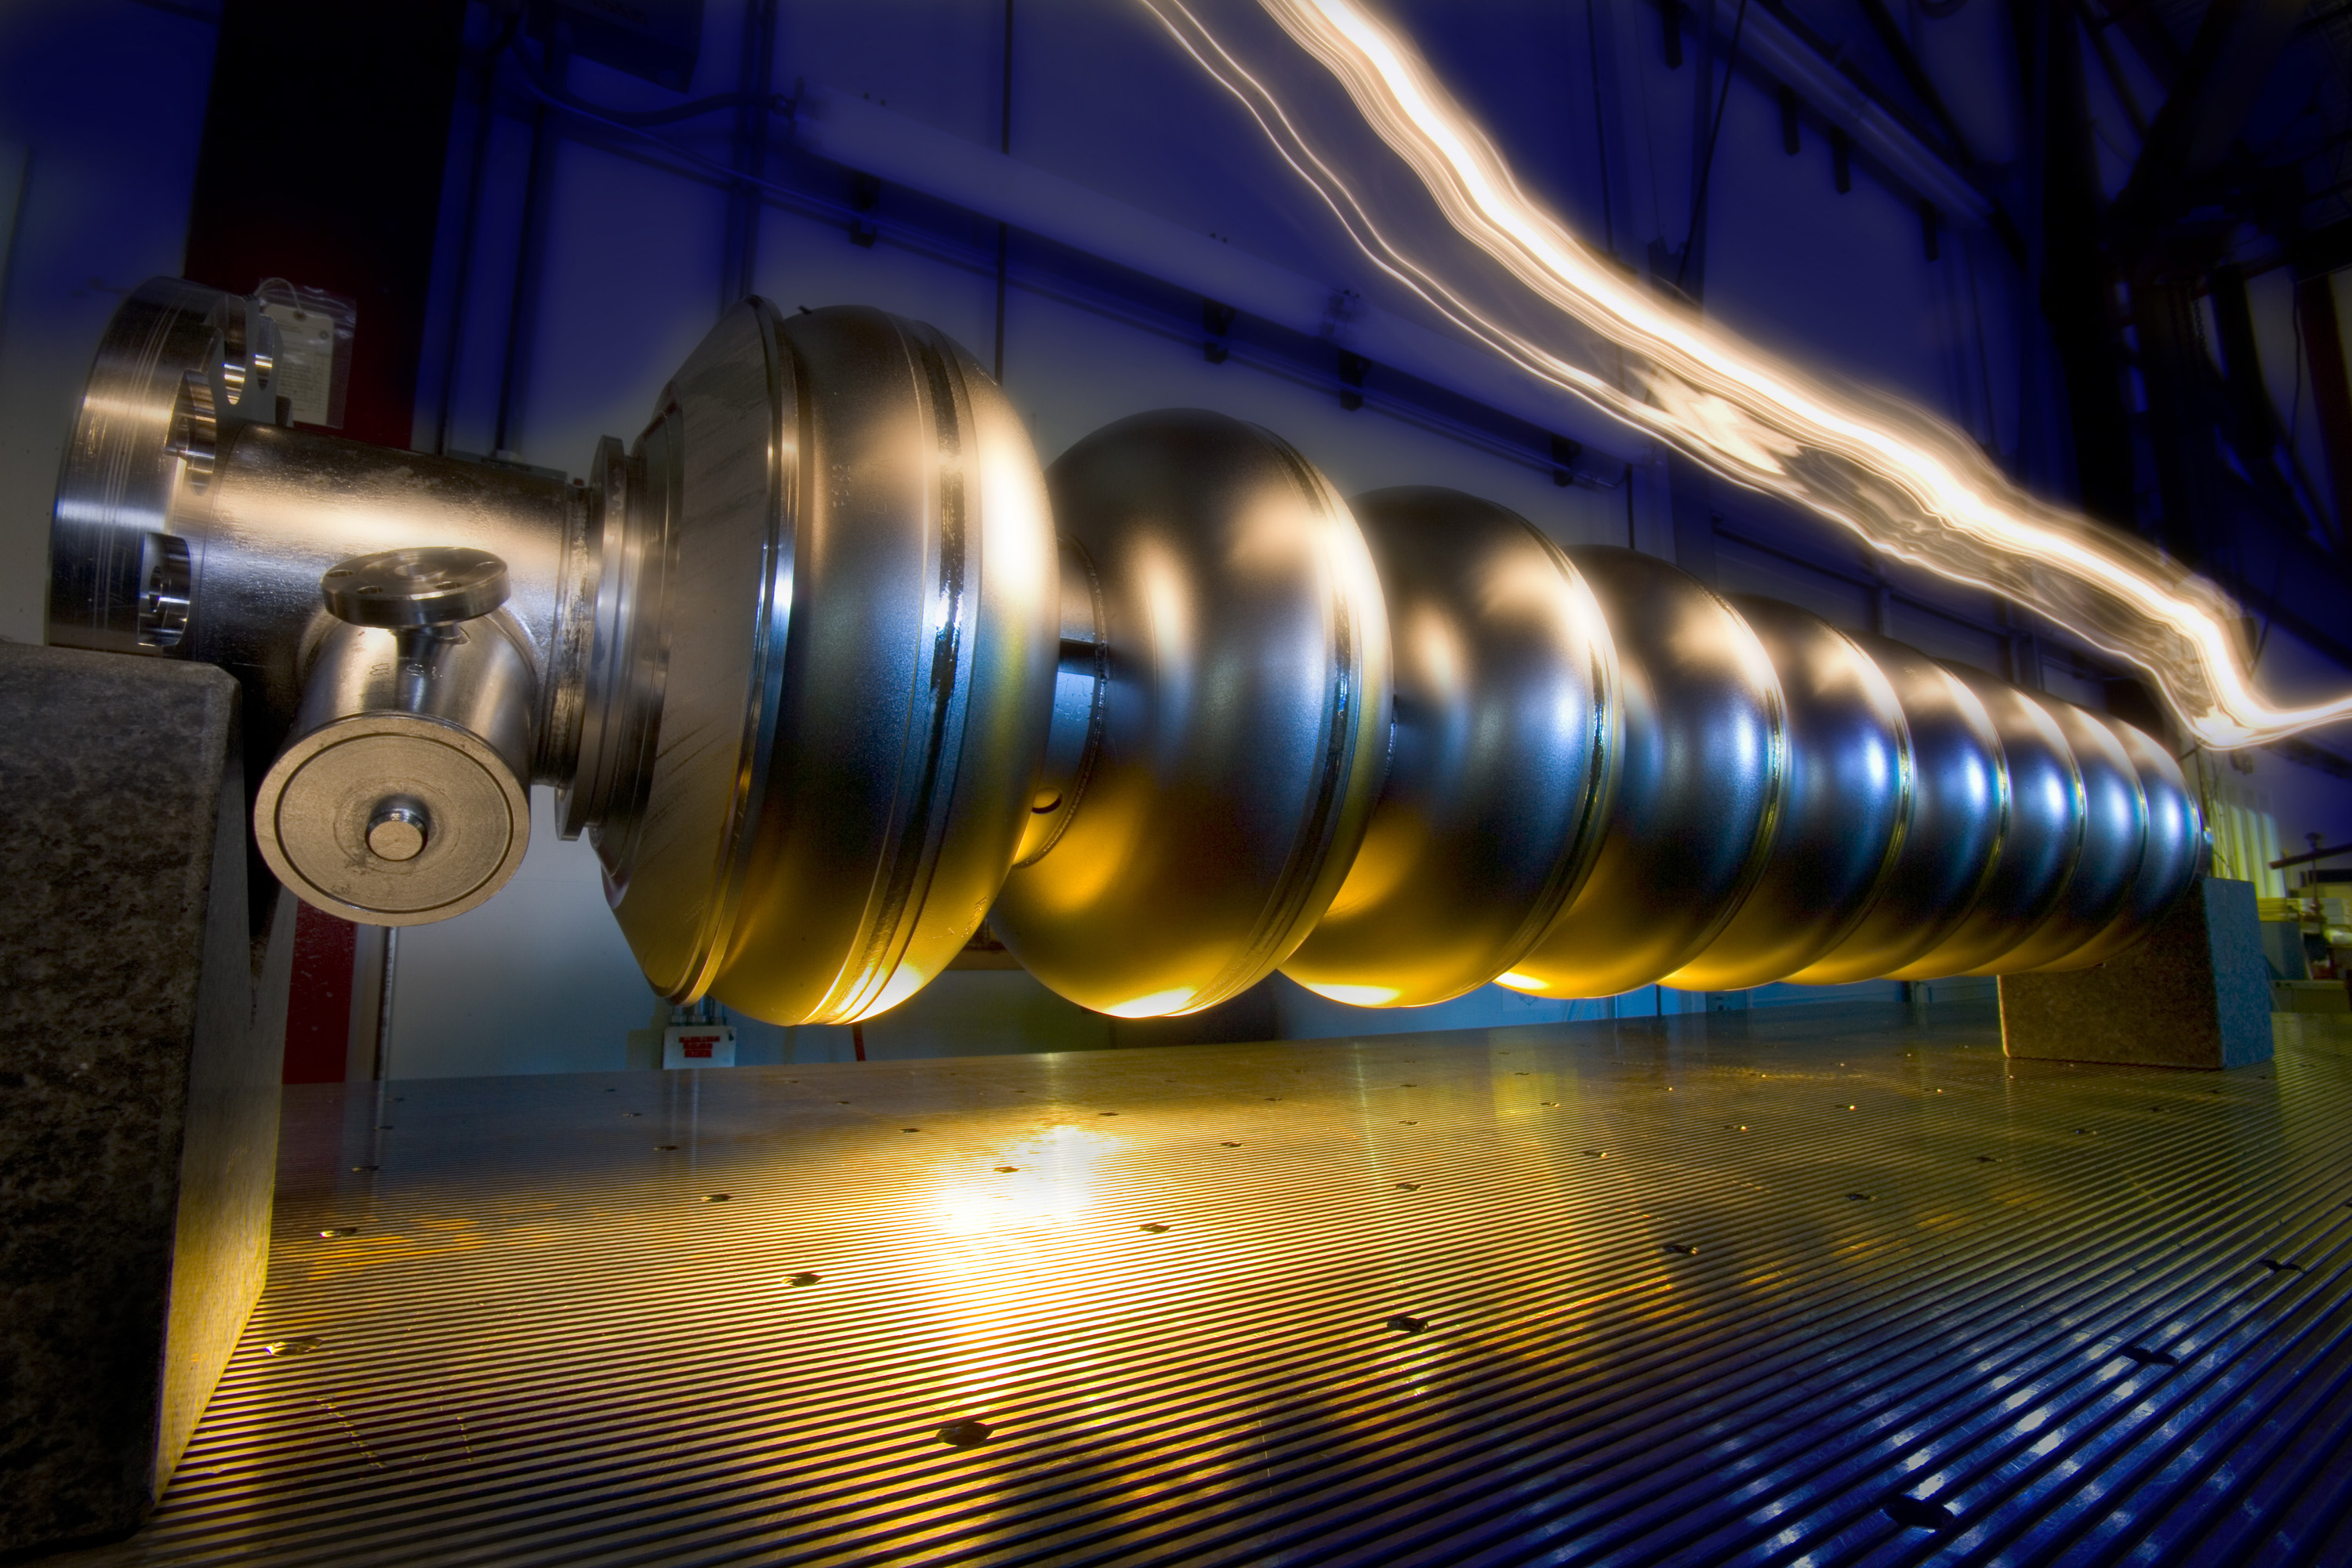
\includegraphics[width=0.45\textwidth]{figures/cavity.jpg}
\end{center}
The cavities are also developed, built and tested at DESY.
\end{frame}

\section{The Final-Focus system}
\begin{frame}{The Final-Focus system}
 \ilclogo
 The Final-Focus (FF) uses:
\begin{itemize}
 \item Strong compact superconducting quadrupoles to focus the
beam at the IP (single collision point with a 14 mrad beam-crossing angle)
\item Sextupoles providing local chromaticity correction
\item Two superconducting octupole doublets, which use nonlinear
focusing to reduce the amplitude of beam-halo particles while leaving the beam core untouched $\rightarrow$ permitting larger collimation amplitude
\item Collimators and spoilers to prevent the beam halo and background particles from entering the detectors
\end{itemize}

\end{frame}


\section{Additional SiD simulation plots}
\begin{frame}{Energy deposition of hits in SiD-EcalEndcaps}
\sidlogo
 \begin{figure}
 \centering
  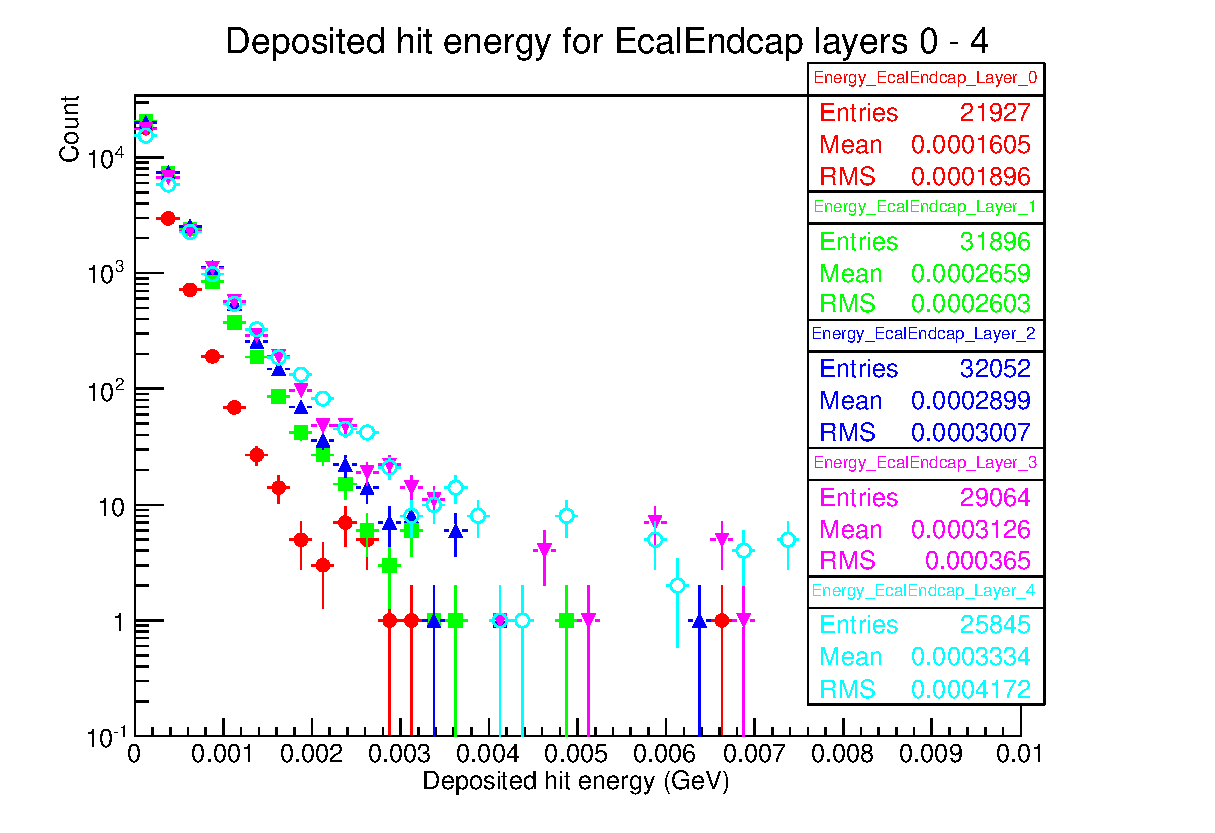
\includegraphics[width=0.6\textwidth]{figures/sidloi3_pairs_1312_EcalEndcap_Hits_EcalEndcap_Energy_EcalEndcap_Layer_0-4.eps}
 \caption{Energy distribution of the hits in the first five layers of the SiD EcalEndcaps}
 \end{figure}
The distributions reach up to about \SI{8}{\mega\electronvolt}.
\end{frame}


\end{document}
